\documentclass[10pt,landscape,a4paper]{article}
\usepackage[english]{babel}
\usepackage[utf8]{inputenc}
\usepackage[plain]{algorithm}
\usepackage[noend]{algpseudocode}
\usepackage{tikz}
\usepackage{pgfplots}
\usepackage{palatino}
\usepackage{multicol}
\usepackage{blkarray}

\usepackage{calc}
\usepackage{ifthen}
\usepackage[landscape]{geometry}
\usepackage{graphicx}
\usepackage{amsmath, amssymb, amsthm}
\DeclareMathOperator*{\argmin}{argmin}
\DeclareMathOperator*{\argmax}{argmax}

\usepackage{physics}
\usepackage{latexsym, marvosym}
\usepackage{pifont}
\usepackage{lscape}
\usepackage{dsfont}
\usepackage{graphicx}
\usepackage{array}
\usepackage{booktabs}
\usepackage[bottom]{footmisc}
\usepackage{tikz}
\usetikzlibrary{shapes}
\usepackage{pdfpages}
\usepackage{wrapfig}
\usepackage{enumitem}
\setlist[description]{leftmargin=0pt}
\usepackage{xfrac}
\usepackage[pdftex,
            pdfauthor={Janus Advincula},
            pdftitle={Machine Learning},
            pdfsubject={A cheatsheet pdf and reference guide made for MIT's 6.86x course.},
            pdfkeywords={machine learning} {statistics} {cheatsheet} {pdf} {cheat} {sheet} {formulas} {equations}
            ]{hyperref}
\usepackage[
            open,
            openlevel=2
            ]{bookmark}
\usepackage{relsize}
\usepackage{rotating}


 \newcommand\independent{\protect\mathpalette{\protect\independenT}{\perp}}
    \def\independenT#1#2{\mathrel{\setbox0\hbox{$#1#2$}%
    \copy0\kern-\wd0\mkern4mu\box0}} 
            
\newcommand{\noin}{\noindent}    
\newcommand{\logit}{\textrm{logit}} 
%\newcommand{\var}{\textrm{Var}}
\newcommand{\cov}{\textrm{Cov}} 
\newcommand{\corr}{\textrm{Corr}} 
\newcommand{\N}{\mathcal{N}}
\newcommand{\Bern}{\textrm{Bern}}
\newcommand{\Bin}{\textrm{Bin}}
\newcommand{\Beta}{\textrm{Beta}}
\newcommand{\Gam}{\textrm{Gamma}}
\newcommand{\Expo}{\textrm{Expo}}
\newcommand{\Pois}{\textrm{Pois}}
\newcommand{\Unif}{\textrm{Unif}}
\newcommand{\Geom}{\textrm{Geom}}
\newcommand{\NBin}{\textrm{NBin}}
\newcommand{\Hypergeometric}{\textrm{HGeom}}
\newcommand{\HGeom}{\textrm{HGeom}}
\newcommand{\Mult}{\textrm{Mult}}

\geometry{top=.4in,left=.2in,right=.2in,bottom=.4in}

\pagestyle{empty}
\makeatletter
\renewcommand{\section}{\@startsection{section}{1}{0mm}%
                                {-1ex plus -.5ex minus -.2ex}%
                                {0.5ex plus .2ex}%x
                                {\normalfont\large\bfseries}}
\renewcommand{\subsection}{\@startsection{subsection}{2}{0mm}%
                                {-1explus -.5ex minus -.2ex}%
                                {0.5ex plus .2ex}%
                                {\normalfont\normalsize\bfseries}}
\renewcommand{\subsubsection}{\@startsection{subsubsection}{3}{0mm}%
                                {-1ex plus -.5ex minus -.2ex}%
                                {1ex plus .2ex}%
                                {\normalfont\small\bfseries}}
\makeatother

\setcounter{secnumdepth}{0}

\setlength{\parindent}{0pt}
\setlength{\parskip}{0pt plus 0.5ex}

% -----------------------------------------------------------------------

\usepackage{titlesec}

\titleformat{\section}
{\color{blue}\normalfont\large\bfseries}
{\color{blue}\thesection}{1em}{}
\titleformat{\subsection}
{\color{violet}\normalfont\normalsize\bfseries}
{\color{violet}\thesection}{1em}{}
% Comment out the above 5 lines for black and white

\begin{document}

\raggedright
\footnotesize
\begin{multicols*}{3}

% multicol parameters
% These lengths are set only within the two main columns
%\setlength{\columnseprule}{0.25pt}
\setlength{\premulticols}{1pt}
\setlength{\postmulticols}{1pt}
\setlength{\multicolsep}{1pt}
\setlength{\columnsep}{2pt}

%%%%%%%%%%%%%%%%%%%%%%%%%%%%%%%%%%%%
%%% TITLE
%%%%%%%%%%%%%%%%%%%%%%%%%%%%%%%%%%%%

\begin{center}
    {\color{blue} \Large{\textbf{6.86x Machine Learning with Python}}} \\
   % {\Large{\textbf{Probability Cheatsheet}}} \\
    % comment out line with \color{blue} and uncomment above line for b&w
\end{center}

%%%%%%%%%%%%%%%%%%%%%%%%%%%%%%%%%%%%
%%% ATTRIBUTIONS
%%%%%%%%%%%%%%%%%%%%%%%%%%%%%%%%%%%%

\scriptsize

This is a cheat sheet for machine learning based on the online course given by Prof. Tommi Jaakkola and Prof. Regina Barzilay. Compiled by Janus B. Advincula.

\begin{center}
    Last Updated \today
\end{center}

% Cheatsheet format from
% http://www.stdout.org/$\sim$winston/latex/

%%%%%%%%%%%%%%%%%%%%%%%%%%%%%%%%%%%%
%%% BEGIN CHEATSHEET
%%%%%%%%%%%%%%%%%%%%%%%%%%%%%%%%%%%%


\section{Linear Classifiers}\smallskip \hrule height 1pt \smallskip

\subsection{Introduction to Machine Learning}

\begin{description}
	\item[What is machine learning?] Machine learning as a discipline aims to design, understand and apply computer programs that learn from experience (i.e., data) for the purpose of modeling, prediction or control.
	\item[Types of Machine Learning] ~
	\begin{itemize}
		\item {\bf Supervised learning:} prediction based on examples of correct behavior
		\item {\bf Unsupervised learning:} no explicit target, only data, goal is to model/discover
		\item {\bf Semi-supervised learning:} supplement limited annotations with unsupervised learning
		\item {\bf Active learning:} learn to query the examples actually needed for learning
		\item {\bf Transfer learning:} how to apply what you have learned from $A$ to $B$
		\item {\bf Reinforcement learning:} learning to act, not just predict; goal is to optimize the consequences of actions
	\end{itemize}
\end{description}

\subsection{Linear Classifier and Perceptron}
\begin{center}
	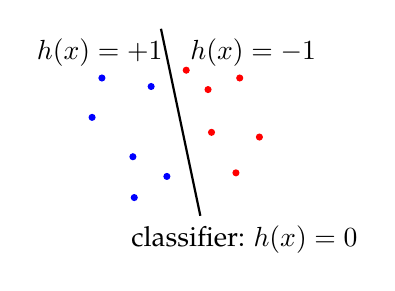
\begin{tikzpicture}[scale=0.5]
	\draw[thick,-] (1,5.25) -- (2,0.5);
	\draw [fill,red] (3,4) circle [radius=0.075];
	\draw [fill,red] (3.5,2.5) circle [radius=0.075];
	\node[below right] at (0,0.5) {classifier: $h(x)=0$};
	\draw [fill, blue] (1.15,1.5) circle [radius=0.075];
	\draw [fill, blue] (-0.5,4) circle [radius=0.075];
	\draw [fill, blue] (-0.75,3) circle [radius=0.075];
	\draw [fill, blue] (0.75,3.7842) circle [radius=0.075];
	\draw [fill, blue] (0.3212,0.963) circle [radius=0.075];
	\draw [fill, red] (2.1954,3.7059) circle [radius=0.075];
	\draw [fill, red] (1.6413,4.1978) circle [radius=0.075];
	\draw [fill, red] (2.2835,2.6196) circle [radius=0.075];
	\draw [fill, blue] (0.2869,2) circle [radius=0.075];
	\draw [fill, red] (2.9040,1.5912) circle [radius=0.075];
	\node[below right] at (-2.4,5.25) {$h(x)=+1$};
	\node[below right] at (1.5,5.25) {$h(x)=-1$};
	\end{tikzpicture}
\end{center}
\begin{description}[itemsep=0pt]
	\item[Key Concepts] ~
	\begin{itemize}
		\item {\bf feature vectors, labels:} $$x\in\mathbb{R}^d,\quad y\in\{-1,+1\}$$
		\item {\bf training set:} $$S_n=\left\{\left(x^{(i)},y^{(i)}\right),i=1,\dots,n\right\}$$
		\item {\bf classifier:} $$h:\mathbb{R}^d\rightarrow\{-1,+1\}$$
		$$\chi^{+}=\left\{x\in\mathbb{R}^d:h(x)=+1\right\}$$
		$$\chi^{-}=\left\{x\in\mathbb{R}^d:h(x)=-1\right\}$$
		\item {\bf training error:} $$\mathcal{E}_n(h)=\frac{1}{n}\sum_{i=1}^{n}\left[\left[h\left(x^{(i)}\right)\neq y^{(i)}\right]\right]$$
		$$\left[\left[h\left(x^{(i)}\right)\neq y^{(i)}\right]\right]=
		\begin{cases}
		1\quad\text{if error}\\
		0\quad\text{otherwise}
		\end{cases}$$
		\item {\bf test error:} $\mathcal{E}(h)$
		\item {\bf set of classifiers:} $h\in\mathcal{H}$
	\end{itemize}
	\item[Linear Classifiers through the Origin] We consider functions of the form
	$$h(x;\theta)=\text{sign}\left(\theta_1x_1+\cdots+\theta_dx_d\right)=\text{sign}\left(\theta\cdot x\right).$$
	\begin{center}
		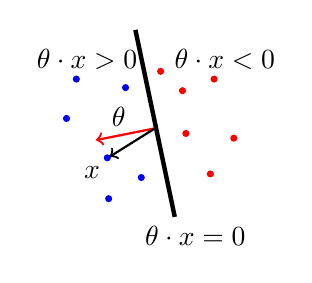
\begin{tikzpicture}[scale=0.5]
		\draw[ultra thick,-] (1,5.25) -- (2,0.5);
		\draw [fill,red] (3,4) circle [radius=0.075];
		\draw [fill,red] (3.5,2.5) circle [radius=0.075];
		\node[below right] at (1,0.5) {$\theta\cdot x=0$};
		\draw[thick, red, ->] (1.5,2.75) -- (0,2.45);
		\draw[thick, ->] (1.5,2.75) -- (0.35,2.03);
		\node[above left] at (1,2.55) {$\theta$};
		\node[below left] at (0.35,2.03) {$x$};
		\draw [fill, blue] (1.15,1.5) circle [radius=0.075];
		\draw [fill, blue] (-0.5,4) circle [radius=0.075];
		\draw [fill, blue] (-0.75,3) circle [radius=0.075];
		\draw [fill, blue] (0.75,3.7842) circle [radius=0.075];
		\draw [fill, blue] (0.3212,0.963) circle [radius=0.075];
		\draw [fill, red] (2.1954,3.7059) circle [radius=0.075];
		\draw [fill, red] (1.6413,4.1978) circle [radius=0.075];
		\draw [fill, red] (2.2835,2.6196) circle [radius=0.075];
		\draw [fill, blue] (0.2869,2) circle [radius=0.075];
		\draw [fill, red] (2.9040,1.5912) circle [radius=0.075];
		\node[below right] at (-1.75,5) {$\theta\cdot x>0$};
		\node[below right] at (1.75,5) {$\theta\cdot x<0$};
		\end{tikzpicture}
	\end{center}
	\item[Linear Classifiers with Offset] We can consider functions of the form $$h(x;\theta)=\text{sign}\left(\theta\cdot x+\theta_0\right)$$
	where $\theta_0$ is the offset parameter.
	\item[Linear Separation] Training examples $S_n$ are {\it linearly separable} if there exists a parameter vector $\widehat{\theta}$ and offset parameter $\widehat{\theta}_0$ such that $y^{(i)}\left(\widehat{\theta}\cdot x^{(i)}+\widehat{\theta}_0\right)>0$ for all $i=1,\dots,n$.
	\item[Training Error] The training error for a linear classifier is
	$$\mathcal{E}_n\left(\theta,\theta_0\right)=\frac{1}{n}\sum_{i=1}^{n}\left[\left[y^{(i)}\left(\theta\cdot x^{(i)}+\theta_0\right)\leq0\right]\right].$$
	\item[Perceptron Algorithm] ~
	\vspace*{-1em}
\begin{algorithm}[H]
{\fontsize{7}{0}
	\begin{algorithmic}
		\Procedure{Perceptron}{$\{(x^{(i)},y^{(i)}),i=1,\dots,n\},T$}
		\State $\theta=0\;\text{(vector)}$
		\For{$t=1,\dots,T$}
			\For{$i=1,\dots,n$}
				\If{$y^{(i)}\left(\theta\cdot x^{(i)}\right)\leq0$}
					\State $\theta=\theta+y^{(i)}x^{(i)}$
				\EndIf
			\EndFor
		\EndFor
		\State \textbf{return} $\theta$
		\EndProcedure
	\end{algorithmic}
}
\end{algorithm}
\vspace*{-3em}

	\item[Perceptron Algorithm (with offset)] ~
	\vspace*{-1em}
\begin{algorithm}[H]
{\fontsize{7}{0}
	\begin{algorithmic}
		\Procedure{Perceptron}{$\{(x^{(i)},y^{(i)}),i=1,\dots,n\},T$}
		\State $\theta=0\;\text{(vector)}$
		\For{$t=1,\dots,T$}
		\For{$i=1,\dots,n$}
		\If{$y^{(i)}\left(\theta\cdot x^{(i)}+\theta_0\right)\leq0$}
		\State $\theta=\theta+y^{(i)}x^{(i)}$
		\State $\theta_0=\theta_0+y^{(i)}$
		\EndIf
		\EndFor
		\EndFor
		\State \textbf{return} $\theta,\theta_0$
		\EndProcedure
	\end{algorithmic}
}
\end{algorithm}
	\vspace*{-3.5em}
	\item[Convergence] Assumptions:
	\begin{itemize}
		\item There exists $\theta^*$ such that $\frac{y^{(i)}\left(\theta^*\cdot x^{(i)}\right)}{\norm{x^{(i)}}}\geq\gamma$ for all $i=1,\dots,n$ for some $\gamma>0.$
		\item All examples are bounded $\norm{x^{(i)}}\leq R$, $i=1,\dots,n.$
	\end{itemize}
	Then the number $k$ of updates made by the perceptron algorithm is bounded by $\dfrac{R^2}{\gamma^2}.$
\end{description}


\subsection{Hinge Loss, Margin Boundaries and Regularization}

\begin{description}
	\item[Distance from a Line to a Point] The perpendicular distance from a line with equation $\theta\cdot x+\theta_0=0$ to a point with coordinates $x_0$ is
	$$d=\dfrac{\left|\theta\cdot x_0+\theta_0\right|}{\lVert\theta\rVert}$$
	\begin{center}
		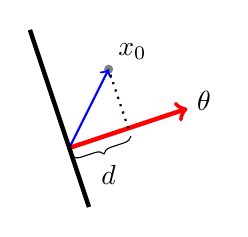
\begin{tikzpicture}[scale=1]
		\draw [fill, gray] (2,2.5) circle [radius=0.05];
		\draw[ultra thick, red, ->] (1.5,1.5) -- (3, 2);
		\draw[thick, blue,->] (1.5, 1.5) -- (2,2.5);
		\node[right] at (3,2.1) {$\theta$};
		\node[above right] at (2,2.5) {$x_0$};
		\draw[ultra thick,-] (1,3) -- (1.75,0.75);
		\draw[dotted, thick] (2.25, 1.75) -- (2,2.5);
		\draw [decorate, decoration={brace,amplitude=3pt,raise=3pt,mirror}] (1.5,1.5) -- (2.25,1.75);
		\node[below] at (2,1.4) {$d$};
		\end{tikzpicture}
	\end{center}
	\item[Decision Boundary] The decision boundary is the set of points $x$ which satisfy $$\theta\cdot x+\theta_0=0.$$
	\item[Margin Boundary] The margin boundary is the set of points $x$ which satisfy $$\theta\cdot x+\theta_0=\pm1.$$
	\begin{center}
		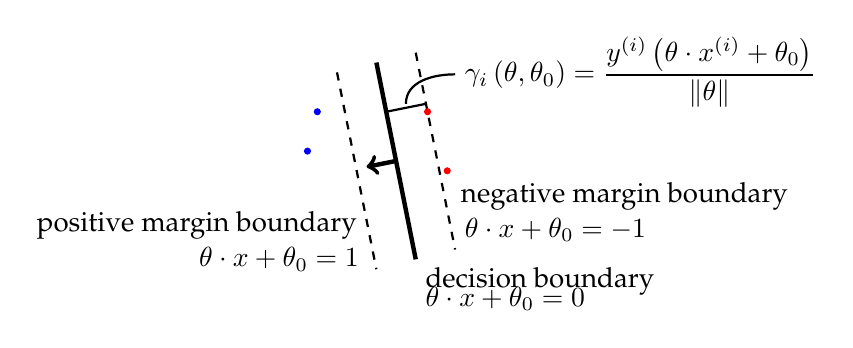
\begin{tikzpicture}[scale=0.5]
		\draw[thick,dashed] (0,5) -- (1,0);
		\draw[ultra thick,-] (1,5.25) -- (2,0.25);
		\draw[thick,dashed] (2,5.5) -- (3,0.5);
		\node[right] at (3,1) {$\theta\cdot x+\theta_0=-1$};
		\node[above right] at (2.9,1.25) {negative margin boundary};
		\node[above left] at (0.75,0.5) {positive margin boundary};
		\node[left] at (0.8,0.25) {$\theta\cdot x +\theta_0=1$};
		\draw [fill,red] (2.3,4) circle [radius=0.075];
		\draw [fill,red] (2.8,2.5) circle [radius=0.075];
		\draw[ultra thick, ->] (1.5,2.75) -- (0.75,2.6);
		\node[below right] at (2,0.3) {decision boundary};
		\node[below right] at (2,-0.2) {$\theta\cdot x+\theta_0=0$};
		\draw [fill, blue] (-0.5,4) circle [radius=0.075];
		\draw [fill, blue] (-0.75,3) circle [radius=0.075];
		\draw[thick, -] (1.25,4) -- (2.25,4.2);
		\draw[thick] (1.75,4.2) to [out=90,in=180] (3,4.95);
		\node[right] at (3,5) {$\gamma_i\left(\theta,\theta_0\right)=\dfrac{y^{(i)}\left(\theta\cdot x^{(i)}+\theta_0\right)}{\norm{\theta}}$};
		\end{tikzpicture}
	\end{center}
	\item[Hinge Loss] ~
	$$\text{Loss}_h\left(z\right)=\begin{cases}
	0&\text{if }z\geq1\\
	1-z&\text{if }z<1
	\end{cases}$$
	with $z=y^{(i)}\left(\theta\cdot x^{(i)}+\theta_0\right)$.
	\item[Regularization] Maximize margin
	$$\max\dfrac{1}{\lVert\theta\rVert}\quad\Rightarrow\quad\min\frac{1}{2}\lVert\theta\rVert^2$$

\end{description}

\subsection{Linear Classification and Generalization}
\begin{center}
	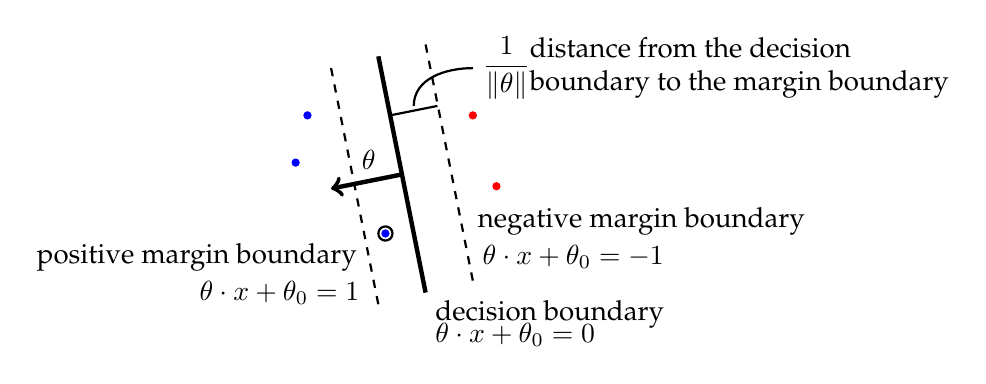
\begin{tikzpicture}[scale=0.6]
	\draw[thick,dashed] (0,5) -- (1,0);
	\draw[ultra thick,-] (1,5.25) -- (2,0.25);
	\draw[thick,dashed] (2,5.5) -- (3,0.5);
	\node[right] at (3,1) {$\theta\cdot x+\theta_0=-1$};
	\node[above right] at (2.9,1.25) {negative margin boundary};
	\node[above left] at (0.75,0.5) {positive margin boundary};
	\node[left] at (0.8,0.25) {$\theta\cdot x +\theta_0=1$};
	\draw [fill,red] (3,4) circle [radius=0.075];
	\draw [fill,red] (3.5,2.5) circle [radius=0.075];
	\draw[ultra thick, ->] (1.5,2.75) -- (0,2.45);
	\node[above left] at (1.15,2.65) {$\theta$};
	\node[below right] at (2,0.3) {decision boundary};
	\node[below right] at (2,-0.2) {$\theta\cdot x+\theta_0=0$};
	\draw [fill, blue] (1.15,1.5) circle [radius=0.075];
	\draw [fill, blue] (-0.5,4) circle [radius=0.075];
	\draw [fill, blue] (-0.75,3) circle [radius=0.075];
	\draw [thick] (1.15,1.5) circle [radius=0.15];
	\draw[thick, -] (1.25,4) -- (2.25,4.2);
	\draw[thick] (1.75,4.2) to [out=90,in=180] (3,5);
	\node[right] at (3,5) {$\dfrac{1}{\norm{\theta}}$};
	\node[right, align=left] at (4,5) {distance from the decision \\ boundary to the margin boundary};
	\end{tikzpicture}
\end{center}


\begin{description}
	\item[Objective function] ~
	$$J\left(\theta,\theta_0\right)=\frac{1}{n}\sum_{i=1}^{n}\left[\text{Loss}_h\left(y^{(i)}\left(\theta\cdot x^{(i)}+\theta_0\right)\right)+\frac{\lambda}{2}\lVert\theta\rVert^2\right]$$
	$\lambda$ is the regularization factor.
	\item[Stochastic Gradient Descent] Select $i\in\{1,\dots,n\}$ at random
	$$\theta\quad\leftarrow\quad\theta-\eta_t\nabla_\theta\left[\text{Loss}_h\left(\theta\cdot x^{(i)}+\theta_0\right)+\frac{\lambda}{2}\lVert\theta\rVert^2\right]$$
	$\eta_t$ is the learning rate which can vary at every iteration.
	\item[Support Vector Machine] ~
	\begin{itemize}
		\item Support Vector Machine finds the maximum margin linear separator by solving the quadratic program that corresponds to $J(\theta,\theta_0)$
		\item In the realizable case, if we disallow any margin violations, the quadratic program we have to solve is:
		
		\hspace*{1cm}Find $\theta,\theta_0$ that minimize $\frac{1}{2}\lVert\theta\rVert^2$ subject to
		$$y^{(i)}\left(\theta\cdot x^{(i)}+\theta_0\right)\geq1,\quad i=1,\dots,n$$
	\end{itemize}
\end{description}
\section{Nonlinear Classification, Linear Regression, \newline Collaborative Filtering} \smallskip \hrule height 1pt \smallskip

\subsection{Linear Regression}

\begin{description}
	\item[Empirical Risk] ~
	$$R_n\left(\theta\right)=\frac{1}{n}\sum_{i=1}^{n}\frac{1}{2}\left(y^{(i)}-\theta\cdot x^{(i)}\right)^2\qquad\text{squared error}$$
	\item[Gradient-based Approach] We can use stochastic gradient descent to find the minima of the empirical risk.\\
	\vspace{0.25cm}
	\hspace*{0.5cm}{\bf Algorithm} \hspace*{0.5cm}Initialize $\theta=0$.\\
	\hspace*{2.25cm}Randomly pick $i=\{1,\dots,n\}$.\\
	\hspace*{2.25cm}$\theta=\theta+\eta\left(y^{(i)}-\theta\cdot x^{(i)}\right)x^{(i)}$.
	
	$\eta$ is the learning rate.
	\item[Closed Form Solution] ~
	Let $$A=\frac{1}{n}\sum_{i=1}^{n}x^{(i)}\left(x^{(i)}\right)^\intercal\quad\text{and}\quad B=\frac{1}{n}\sum_{i=1}^{n}y^{(i)}x^{(i)}.$$ Then,
	$$\widehat{\theta}=A^{-1}B.$$ In matrix notation, this is
	$$\widehat{\theta}=\left(\mathbb{X}^\intercal\mathbb{X}\right)^{-1}\mathbb{X}^\intercal\mathbb{Y}.$$
	\item[Generalization and Regularization] ~
	
	{\bf Ridge Regression:} The loss function is $$J_{\lambda,n}=\frac{\lambda}{2}\norm{\theta}^2+R_n\left(\theta\right)$$
	where $\lambda$ is the regularization factor. We can find its minima using gradient-based approach.\\
	\vspace{0.25cm}
	\hspace*{0.5cm}{\bf Algorithm} \hspace*{0.5cm}Initialize $\theta=0$.\\
	\hspace*{2.25cm}Randomly pick $i=\{1,\dots,n\}$.\\
	\hspace*{2.25cm}$\theta=\left(1-\eta\lambda\right)\theta+\eta\left(y^{(i)}-\theta\cdot x^{(i)}\right)x^{(i)}$.
\end{description}

\subsection{Nonlinear Classification}
\begin{description}
	\item[Feature Transformation] ~
	\begin{align*}
		x&\mapsto\phi(x)\\
		\theta\cdot x&\rightarrow\theta'\cdot\phi(x)
	\end{align*}
	\item[Non-linear Classification] ~
	$$h\left(x;\theta,\theta_0\right)=\text{sign}\left(\theta\cdot\phi(x)+\theta_0\right)$$
	\item[Kernel Function] A kernel function is simply an inner product between two feature vectors. Using kernels is advantageous when the inner products are faster to evaluate than using explicit vectors (e.g., when the vectors would be infinite dimensional).
	$$K\left(x,x'\right)=\phi(x)\cdot\phi(x')$$
	\item[Perceptron] ~
	\vspace*{-1em}
	\begin{algorithm}[H]
		{\fontsize{7}{0}
			\begin{algorithmic}
				\State $\theta=0$
				\For{$i=1,\dots,n$}
				\If{$y^{(i)}\theta\cdot\phi\left(x^{(i)}\right)\leq0$}
				\State $\theta\leftarrow\theta+y^{(i)}\phi\left(x^{(i)}\right)$
				\EndIf
				\EndFor
			\end{algorithmic}
		}
	\end{algorithm}
	\vspace*{-3em}
	This algorithm gives
	$$\theta=\sum_{j=1}^{n}\alpha_jy^{(j)}\phi\left(x^{(j)}\right)$$
	where $\alpha_j$ is the number of mistakes. For the offset parameter, we get
	$$\theta_0=\sum_{j=1}^{n}\alpha_jy^{(j)}.$$
	\item[Kernel Perceptron Algorithm] We can reformulate the perceptron algorithm so that we initialize and update $\alpha_j$'s, instead of $\theta$.
	$$\theta\cdot\phi\left(x^{(i)}\right)=\sum_{j=1}^{n}\alpha_jy^{(j)}\underbrace{\phi\left(x^{(j)}\right)\cdot\phi\left(x^{(i)}\right)}_{K\left(x^{(j)},x^{(i)}\right)}$$
	\vspace*{-2em}
	\begin{algorithm}[H]
		{\fontsize{7}{0}
			\begin{algorithmic}
				\Procedure{Kernel Perceptron}{$\{(x^{(i)},y^{(i)}),i=1,\dots,n\},T$}
				\State \textbf{Initialize} $\alpha_1,\dots,\alpha_n \text{ to some values}$
				\For{$t=1,\dots,T$}
				\For{$i=1,\dots,n$}
				\If{$y^{(i)}\sum\limits_{j=1}^{n}\alpha_jy^{(j)}K\left(x^{(j)},x^{(i)}\right)\leq0$}
				\State $\alpha_j=\alpha_j+1$
				\EndIf
				\EndFor
				\EndFor
				\EndProcedure
			\end{algorithmic}
		}
	\end{algorithm}
	\vspace*{-2em}
	The initilization $\theta=0$ is equivalent to $\alpha_1=\dots=\alpha_n=0$.
	\item[Composition rules:] ~
	\begin{enumerate}
		\item $K(x,x')=1$ is a kernel function.
		\item Let $f:\mathbb{R}^d\rightarrow\mathbb{R}$ and $K(x,x')$ is a kernel. Then so is $\widetilde{K}(x,x')=f(x)K(x,x')f(x')$
		\item If $K_1(x,x')$ and $K_2(x,x')$ are kernels, then $K(x,x')=K_1(x,x')+K_2(x,x')$ is a kernel.
		\item If $K_1(x,x')$ and $K_2(x,x')$ are kernels, then $K(x,x')=K_1(x,x')K_2(x,x')$ is a kernel.
	\end{enumerate}
	\item[Decision Boundary] The decision boundary satisfies
	$$\sum_{j=1}^{n}\alpha_jy^{(j)}K\left(x^{(j)},x\right)=0.$$
	\item[Radial Basis Kernel] ~
	$$K(x,x')=\exp(-\frac{1}{2}\norm{x-x'}^2)$$
	\begin{center}
		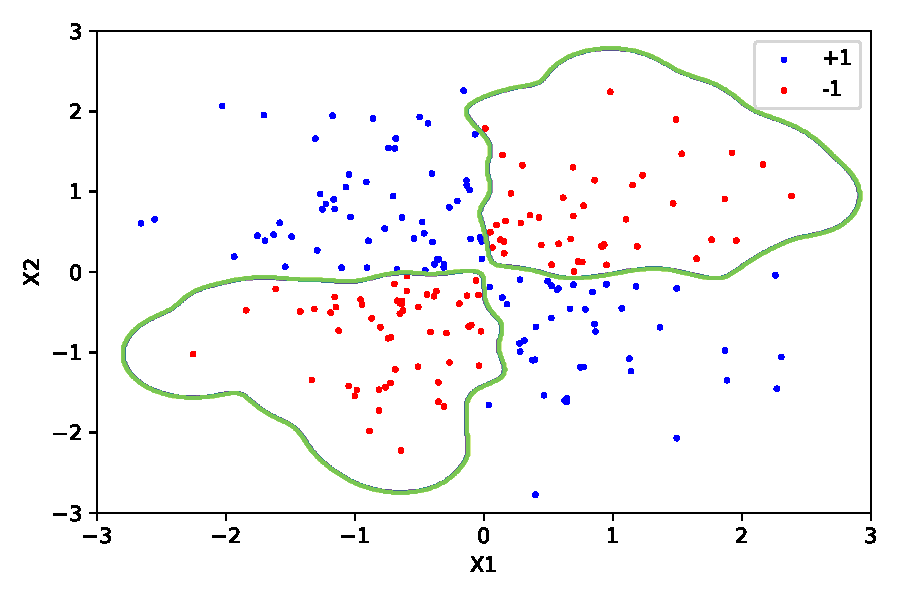
\includegraphics[width=0.6\columnwidth]{rbf.pdf}
	\end{center}
	\item[Other non-linear classifiers] ~
	\begin{itemize}
		\item We can get non-linear classifiers or regression methods by simply mapping examples into feature vectors non-linearly, and applying a linear method on the resulting vectors.
		\item These feature vectors can be high dimensional.
		\item We can turn the linear methods into kernel methods by casting the computations in terms of inner products.
	\end{itemize}
\end{description}

\subsection{Recommender Systems}

\begin{description}
	\item[Problem Description] We are given a matrix where each row corresponds to a user's rating of movies, for example, and each column corresponds to the user ratings for a particular movie. It can also be product ratings, etc. This matrix will be very sparse. The goal is to predict user ratings for those movies that are yet to be rated.
	\[
	\begin{blockarray}{cccc}
	& & m\text{ movies} \\
	\begin{block}{c(ccc)}
	 &  &  &  \\
	 &  &  &  \\
	n \text{ users}   &  & Y_{ai} & \\
	 &  &  & \\
	 &  &  & \\
	\end{block}
	\end{blockarray}
	\]
	\vspace*{-2em}
	\item[$K$-Nearest Neighbor Method] The $K$-Nearest Neighbor method makes use of ratings by $K$ other {\it similar} users when predicting $Y_{ai}.$ Let $\text{KNN}(a)$ be the set of $K$ users {\it similar to} user $a$, and let $\text{sim}(a,b)$ be a {\bf similarity measure} between users $a$ and $b\in\text{KNN}(a).$ The KNN method predicts a rating $Y_{ai}$ to be
	$$\widehat{Y}_{ai}=\dfrac{\sum\limits_{b\in\text{KNN}(a)}\text{sim}(a,b)Y_{bi}}{\sum\limits_{b\in\text{KNN}(a)}\text{sim}(a,b)}$$
	The similarity measure $\text{sim}(a,b)$ could be any distance function between the feature vectors $x_a$ and $x_b$.
	\begin{itemize}
		\item Euclidean distance: $\norm{x_a-x_b}$
		\item Cosine similarity: $\cos\theta=\dfrac{x_a\cdot x_b}{\norm{x_a}\norm{x_b}}$
	\end{itemize}
	\item[Collaborative Filtering] Our goal is to come up with a matrix $X$ that has no blank entries and whose $(a,i)$\textsuperscript{th} entry $X_{ai}$ is the prediction of user $a$'s rating to movie $i$.
	
	Let $D$ be the set of all $(a,i)$'s for which a user rating $Y_{ai}$ exists. A naive approach is to minimize the objective function
	$$J(X)=\sum_{(a,i)\in D}\frac{1}{2}\left(Y_{ai}-X_{ai}\right)^2+\frac{\lambda}{2}\sum_{(a,i)}X_{ai}^2.$$
	The results are
	\begin{align*}
		\widehat{X}_{ai}&=\dfrac{Y_{ai}}{1+\lambda}\quad\text{for }(a,i)\in D\\
		\widehat{X}_{ai}&=0\qquad\quad\;\,\text{for }(a,i)\notin D.
	\end{align*}
	The problem with this approach is that there is no connection between the entries of $X$. We can impose additional constraint on $X$: $$X=UV^\intercal$$
	for some $n\times d$ matrix $U$ and $d\times m$ matrix $V^\intercal$, where $d$ is the {\it rank} of the matrix $X$.
	\item[Alternating Minimization] Assume that $U$ and $V$ are rank $k$ matrices. Then, we can write the objective function as
	$$J(X)=\sum_{(a,i)\in D}\frac{1}{2}\left(Y_{ai}-\left[UV^\intercal\right]_{ai}\right)^2+\frac{\lambda}{2}\left(\sum_{a,k}U_{ak}^2+\sum_{i,k}V_{ik}^2\right).$$
	To find the solution, we fix (initialize) $U$ (or $V$) and minimize the objective with respect to $V$ (or $U$). We plug-in the result back to the objective and minimize it with respect to $U$ (or $V$). We repeat this alternating process until there is no change in the objective function.
	\item[Example] Consider the case $k=1$. Then, $U_{a1}=u_a$ and $V_{i1}=v_i$. If we initialize $u_a$ to some values, then we have to optimize the function
	$$\sum_{(a,i)\in D}\frac{1}{2}\left(Y_{ai}-u_av_i\right)^2+\frac{\lambda}{2}\sum_{i}v_{i}^2.$$
\end{description}

\section{Neural Networks}\smallskip \hrule height 1pt \smallskip

\subsection{Introduction to Feedforward Neural Networks}

\begin{description}
	\item[A Unit in a Neural Network] A {\bf neural network unit} is a primitive neural network that consists of only the {\it input layer}, and an output layer with only one output.
	\begin{center}
		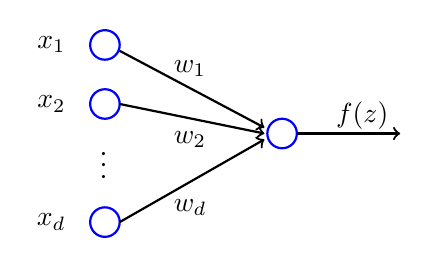
\begin{tikzpicture}[scale=0.75]
		\draw[thick,blue] (0,0) circle [radius=0.25];
		\draw[thick,blue] (0,2) circle [radius=0.25];
		\draw[thick,blue] (0,3) circle [radius=0.25];
		\node[left] at (0.2,1.1) {$\vdots$};
		\node[left] at (-0.5,3) {$x_1$};
		\node[left] at (-0.5,2) {$x_2$};
		\node[left] at (-0.5,0) {$x_d$};
		\draw[thick,blue] (3,1.5) circle [radius=0.25];%
		\draw[thick,->] (0.25,2.9) -- (2.7,1.6);
		\draw[thick,->] (0.25,2) --(2.7,1.5);
		\draw[thick,->] (0.25,0) -- (2.7,1.4);
		\draw[thick,->] (3.25,1.5) -- (5,1.5);
		\node[right] at (1,2.6) {$w_1$};
		\node[right] at (1,1.4) {$w_2$};
		\node[right] at (1,0.25) {$w_d$};
		\node[right] at (3.75,1.8) {$f(z)$};
		\end{tikzpicture}
	\end{center}
	A neural network unit computes a non-linear weighted combination of its input: $$\widehat{y}=f(z)\qquad\text{where}\quad z=w_0+\sum_{i=1}^{d}x_iw_i$$
	where $w_i$ are the {\bf weights}, $z$ is a number and is the weighted sum of the inputs $x_i$, and $f$ is generally a non-linear function called the {\bf activation function}.
	\item[Linear Function] $f(z)=z$
	\item[Rectified Linear Unit (ReLU)] $f(z)=\max\{0,z\}$
	\item[Hyperbolic Tangent Function] $\tanh(z)=\dfrac{e^z-e^{-z}}{e^z+e^{-z}}=1-\dfrac{2}{e^{2z}+1}$
	\item[Deep Neural Networks] A {\bf deep (feedforward) neural network} refers to a neural network that contains not only the input and output layers, but also hidden layers in between. Below is a deep feedforward neural network of 2 hidden layers, with each hidden layer consisting of 5 units:
	\begin{center}
		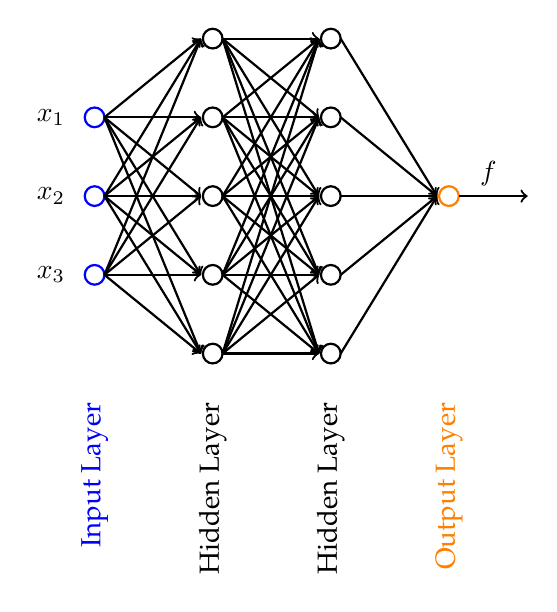
\begin{tikzpicture}[scale=0.5]
		\draw[thick,blue] (0,0) circle [radius=0.25];
		\draw[thick,blue] (0,2) circle [radius=0.25];
		\draw[thick,blue] (0,4) circle [radius=0.25];
		\node[left] at (-0.5,4) {$x_1$};
		\node[left] at (-0.5,2) {$x_2$};
		\node[left] at (-0.5,0) {$x_3$};
		\draw[thick] (3,6) circle [radius=0.25];
		\draw[thick] (3,4) circle [radius=0.25];
		\draw[thick] (3,2) circle [radius=0.25];
		\draw[thick] (3,0) circle [radius=0.25];
		\draw[thick] (3,-2) circle [radius=0.25];
		\draw[thick] (6,6) circle [radius=0.25];
		\draw[thick] (6,4) circle [radius=0.25];
		\draw[thick] (6,2) circle [radius=0.25];
		\draw[thick] (6,0) circle [radius=0.25];
		\draw[thick] (6,-2) circle [radius=0.25];
		\draw[thick,orange] (9,2) circle [radius=0.25];
		\node[above] at (10,2) {$f$};
		\node[left, rotate=90, blue] at (0,-3) {Input Layer};
		\node[left, rotate=90] at (3,-3) {Hidden Layer};
		\node[left, rotate=90] at (6,-3) {Hidden Layer};
		\node[left, rotate=90, orange] at (9,-3) {Output Layer};
		\draw[thick,->] (9.25,2) -- (11,2);
		\draw[thick,->] (0.25,4) -- (2.7,6);
		\draw[thick,->] (0.25,4) -- (2.7,4);
		\draw[thick,->] (0.25,4) -- (2.7,2);
		\draw[thick,->] (0.25,4) -- (2.7,0);
		\draw[thick,->] (0.25,4) -- (2.7,-2);
		\draw[thick,->] (0.25,2) --(2.7,6);
		\draw[thick,->] (0.25,2) --(2.7,4);
		\draw[thick,->] (0.25,2) --(2.7,2);
		\draw[thick,->] (0.25,2) --(2.7,0);
		\draw[thick,->] (0.25,2) --(2.7,-2);
		\draw[thick,->] (0.25,0) -- (2.7,6);
		\draw[thick,->] (0.25,0) -- (2.7,4);
		\draw[thick,->] (0.25,0) -- (2.7,2);
		\draw[thick,->] (0.25,0) -- (2.7,0);
		\draw[thick,->] (0.25,0) -- (2.7,-2);
		\draw[thick,->] (3.25,-2) -- (5.7,6);
		\draw[thick,->] (3.25,-2) -- (5.7,4);
		\draw[thick,->] (3.25,-2) -- (5.7,2);
		\draw[thick,->] (3.25,-2) -- (5.7,0);
		\draw[thick,->] (3.25,-2) -- (5.7,-2);
		\draw[thick,->] (3.25,0) -- (5.7,6);
		\draw[thick,->] (3.25,0) -- (5.7,4);
		\draw[thick,->] (3.25,0) -- (5.7,2);
		\draw[thick,->] (3.25,0) -- (5.7,0);
		\draw[thick,->] (3.25,0) -- (5.7,-2);
		\draw[thick,->] (3.25,2) -- (5.7,6);
		\draw[thick,->] (3.25,2) -- (5.7,4);
		\draw[thick,->] (3.25,2) -- (5.7,2);
		\draw[thick,->] (3.25,2) -- (5.7,0);
		\draw[thick,->] (3.25,2) -- (5.7,-2);
		\draw[thick,->] (3.25,4) -- (5.7,6);
		\draw[thick,->] (3.25,4) -- (5.7,4);
		\draw[thick,->] (3.25,4) -- (5.7,2);
		\draw[thick,->] (3.25,4) -- (5.7,0);
		\draw[thick,->] (3.25,4) -- (5.7,-2);
		\draw[thick,->] (3.25,6) -- (5.7,6);
		\draw[thick,->] (3.25,6) -- (5.7,4);
		\draw[thick,->] (3.25,6) -- (5.7,2);
		\draw[thick,->] (3.25,6) -- (5.7,0);
		\draw[thick,->] (3.25,6) -- (5.7,-2);
		\draw[thick,->] (6.25,6) -- (8.7,2);
		\draw[thick,->] (6.25,4) -- (8.7,2);
		\draw[thick,->] (6.25,2) -- (8.7,2);
		\draw[thick,->] (6.25,0) -- (8.7,2);
		\draw[thick,->] (6.25,-2) -- (8.7,2);
		\end{tikzpicture}
	\end{center}
	\item[One Hidden Layer Model] ~
	\begin{center}
		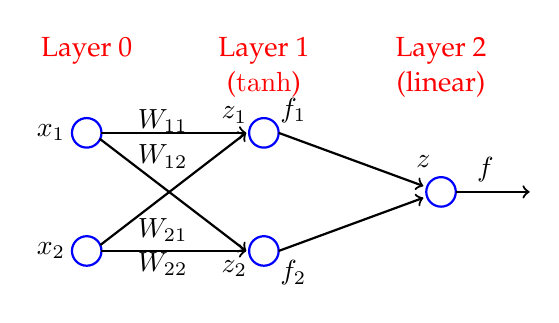
\begin{tikzpicture}[scale=0.75]
		\draw[thick,blue] (0,0) circle [radius=0.25];
		\draw[thick,blue] (0,2) circle [radius=0.25];
		\node[left] at (-0.2,2) {$x_1$};
		\node[left] at (-0.2,0) {$x_2$};
		\draw[thick,blue] (3,2) circle [radius=0.25];
		\draw[thick,blue] (3,0) circle [radius=0.25];
		\draw[thick,blue] (6,1) circle [radius=0.25];
		\draw[thick,->] (6.25,1) -- (7.5,1);
		\draw[thick,->] (0.25,2) --(2.7,2);
		\draw[thick,->] (0.22,1.9) --(2.7,0);
		\draw[thick,->] (0.25,0) -- (2.7,0);
		\draw[thick,->] (0.23,0.1) -- (2.7,2);
		\node[right] at (0.7,2.2) {$W_{11}$};
		\node[right] at (0.7,1.6) {$W_{12}$};
		\node[right] at (0.7,0.35) {$W_{21}$};
		\node[right] at (0.7,-0.22) {$W_{22}$};
		\draw[thick,->] (3.25,2) -- (5.7,1.1);
		\draw[thick,->] (3.25,0) -- (5.7,0.9);
		\node[above] at (6.75,1) {$f$};
		\node[above] at (5.7,1.25) {$z$};
		\node[above] at (2.5,2) {$z_1$};
		\node[above] at (3.5,2) {$f_1$};
		\node[below] at (2.5,0) {$z_2$};
		\node[below] at (3.5,0) {$f_2$};
		\node[above,red] at (0,3) {Layer 0};
		\node[above,red] at (3,3) {Layer 1};
		\node[below,red] at (3,3.2) {($\tanh$)};
		\node[above,red] at (6,3) {Layer 2};
		\node[below,red] at (6,3.2) {(linear)};
		\end{tikzpicture}
	\end{center}
	\begin{alignat*}{3}
		z_1&=\sum_{j=1}^{2}x_jW_{j1}+W_{01}\qquad		&&z_2&&=\sum_{j=1}^{2}x_jW_{j2}+W_{02}\\
		f_1&=f(z_1)=\tanh(z_1)\qquad &&f_2&&=f(z_2)=\tanh(z_2)\\
		z&=f_1w'_1+f_2w'_2 &&f&&=f(z)=z
	\end{alignat*}
	\item[Neural Signal Transformation] We can visualize what the hidden layer is doing similarly to a linear classifier.
	\begin{center}
		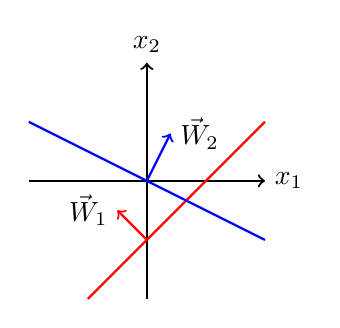
\begin{tikzpicture}[scale=0.75]
		\node[right] at (2,0) {$x_1$};
		\node[above] at (0,2) {$x_2$};
		\draw[thick,->] (-2,0) -- (2,0);
		\draw[thick,->] (0,-2) --(0,2);
		\draw[thick,red,->] (0,-1) --(-0.5,-0.5);
		\draw[thick,red] (-1,-2) --(2,1);
		\node[left] at (-0.5,-0.5) {$\vec{W}_1$};
		\draw[thick,blue] (2,-1) --(-2,1);
		\draw[thick,blue,->] (0,0) --(0.4,0.8);
		\node[right] at (0.4,0.8) {$\vec{W}_2$};
		\end{tikzpicture}
	\end{center}
	In the figure, $$\vec{W}_1=\begin{pmatrix}
	W_{11}\\
	W_{21}
	\end{pmatrix}\qquad\text{and}\quad\vec{W}_2=\begin{pmatrix}
	W_{12}\\
	W_{22}
	\end{pmatrix}.$$
	They map the input onto the $f_1$-$f_2$ axes.
\end{description}

\begin{description}
	\item[Hidden Layer Representation] ~
	\begin{itemize}[noitemsep, topsep=0pt]
		\item Hidden Layer Units
		\begin{center}
			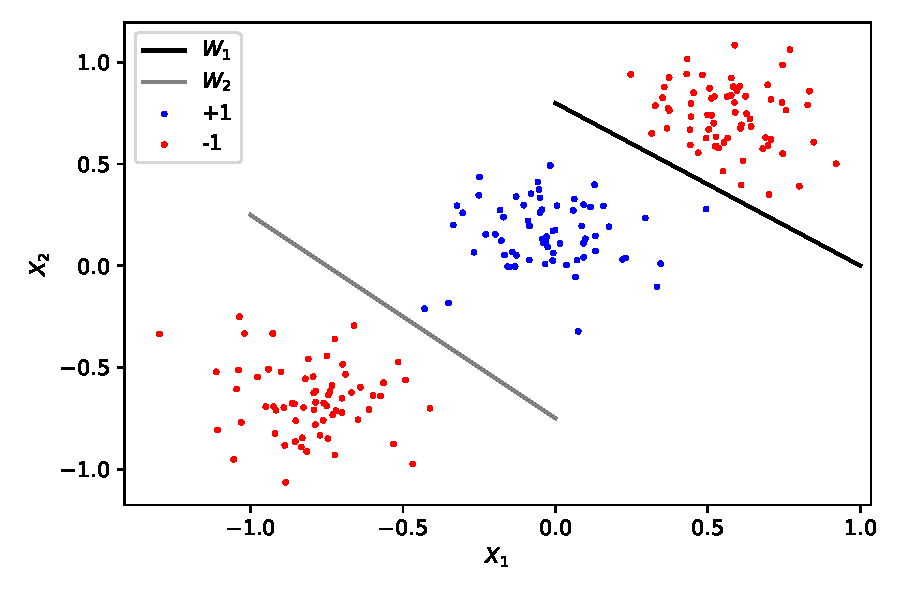
\includegraphics[width=0.6\columnwidth]{data.pdf}
		\end{center}
		\item Linear Activation
		\begin{center}
			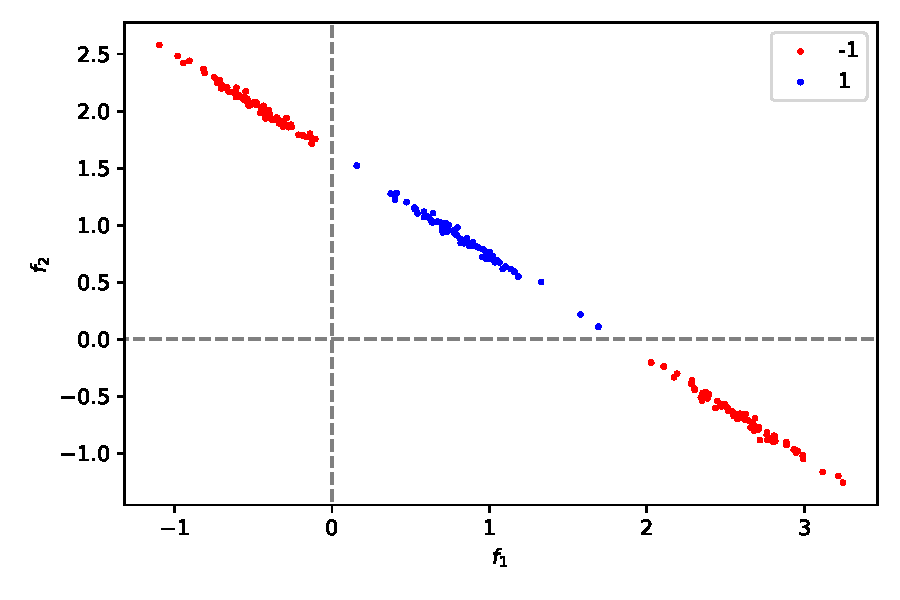
\includegraphics[width=0.6\columnwidth]{linear.pdf}
		\end{center}
		\item $tanh$ Activation
		\begin{center}
			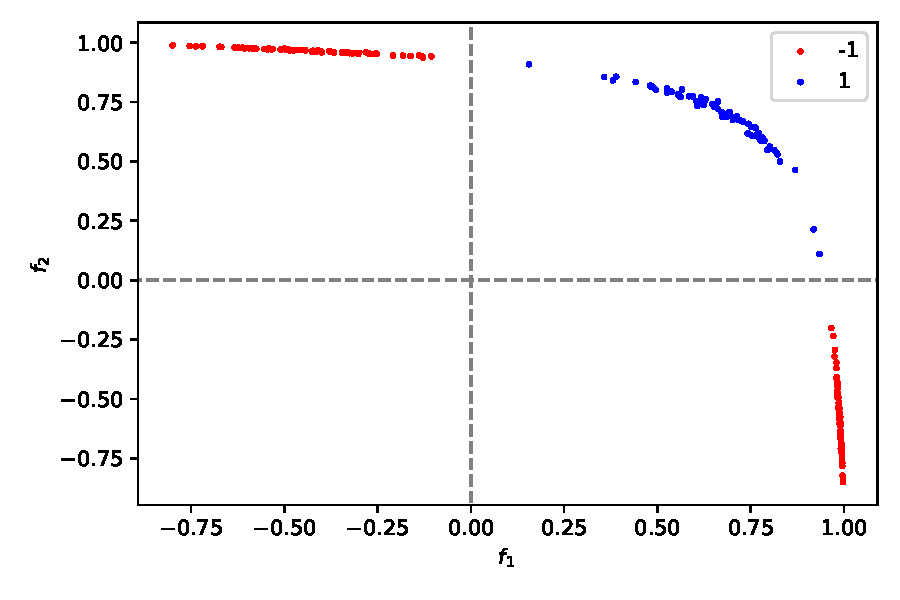
\includegraphics[width=0.6\columnwidth]{tanh.pdf}
		\end{center}
		\item ReLU Activation
		\begin{center}
			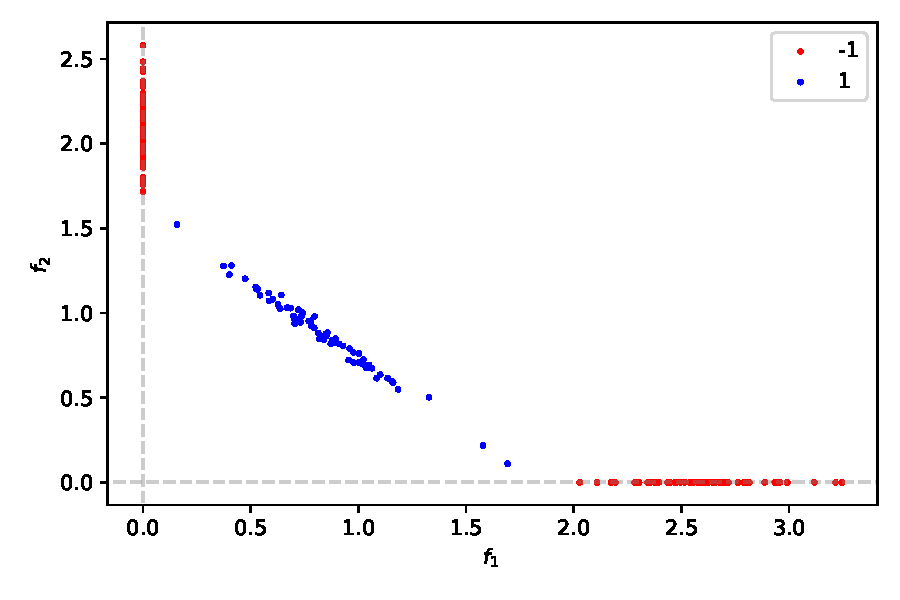
\includegraphics[width=0.6\columnwidth]{relu.pdf}
		\end{center}
	\end{itemize}
	\item[Summary] ~
	\begin{itemize}
		\item Units in neural networks are linear classifiers, just with different output non-linearity.
		\item The units in feedforward neural networks are arranged in layers.
		\item By learning the parameters associated with the hidden layer units, we learn how to represent examples (as hidden layer activations).
		\item The representations in neural networks are learned directly to facilitate the end-to-end task.
		\item A simple classifier (output unit) suffices to solve complex classification tasks if it operates on the hidden layer representations.
	\end{itemize}
\end{description}
\subsection{Feedforward Neural Networks, Back Propagation, and Stochastic Gradient Descent (SGD)}

\begin{description}
	\item[Simple Example] This simple neural network is made up of $L$ hidden layers, but each layer consists of only one unit, and each unit has activation function $f$.
	\begin{center}
	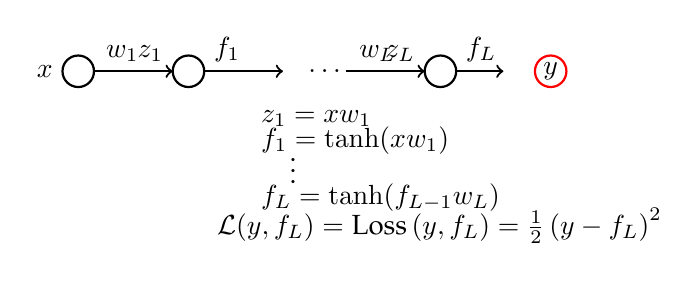
\begin{tikzpicture}[scale=0.8]
	\node[left] at (-0.5,0) {$x$};
	\draw[thick] (-0.25,0) circle [radius=0.25];
	\draw[thick,->] (0,0) -- (1.25,0);
	\node[above] at (0.45,0) {$w_1$};
	\draw[thick] (1.5,0) circle [radius=0.25];
	\node[above left] at (1.25,0) {$z_1$};
	\node[above right] at (1.75,0) {$f_1$};
	\draw[thick,->] (1.75,0) --(3,0);
	\draw[thick,->] (4,0) -- (5.25,0);
	\node[above] at (4.5,0) {$w_L$};
	\node[right] at (3.25,0) {$\dots$};
	\draw[thick] (5.5,0) circle [radius=0.25];
	\node[above left] at (5.25,0) {$z_L$};
	\node[above right] at (5.75,0) {$f_L$};
	\draw[thick,->] (5.75,0) -- (6.5,0);
	\draw[red,thick] (7.25,0) circle [radius=0.25];
	\node at (7.25,0) {$y$};
	\node[right] at (2.5, -0.75) {$z_1=xw_1$};
	\node[right] at (1.8,-2.45) {$\mathcal{L}(y,f_L)=\text{Loss}\left(y,f_L\right)=\frac{1}{2}\left(y-f_L\right)^2$};
	\node[right] at (2.5,-1.1) {$f_1=\tanh(xw_1)$};
	\node[right] at (2.95,-1.45) {$\vdots$};
	\node[right] at (2.5,-2) {$f_L=\tanh(f_{L-1}w_L)$};
	\end{tikzpicture}
	\end{center}
	For $i=2,\dots,L$: $z_i=f_{i-1}w_i$ where $f_{i-1}=f(z_{i-1})$. Also, $y$ is the true value and $f_L$ is the output of the neural network.
	\item[Gradient Descent] The gradient descent update rule for the parameter $w_i$ is
	$$w_i\leftarrow w_i-\eta\cdot\grad_{w_i}{\mathcal{L}(y,f_L)}$$
	where $\eta$ is the learning rate. For instance, we have
	\begin{align*}
		\dfrac{\partial\mathcal{L}}{\partial w_1}&=\dfrac{\partial f_1}{\partial w_1}\dfrac{\partial\mathcal{L}}{\partial f_1}\\
		\dfrac{\partial f_1}{\partial w_1}&=\left[1-\tanh^2(xw_1)\right]x=\left(1-f_1^2\right)x\\
		\dfrac{\partial\mathcal{L}}{\partial f_1}&=\dfrac{\partial\mathcal{L}}{\partial f_2}\dfrac{\partial f_2}{\partial f_1}=\dfrac{\partial\mathcal{L}}{\partial f_2}\left(1-f_2^2\right)w_2.
	\end{align*}
	Thus, when we back-propagate, we get
	$$\dfrac{\partial\mathcal{L}}{\partial w_1}=x\left(1-f_1^2\right)\cdots\left(1-f_L^2\right)w_2\cdots w_L\cdot2\left(f_L-y\right).$$
	Note that the above derivation applies to $\tanh$ activation.
	\item[Backpropagation] Consider the $L$-layer neural network below.
	\begin{center}
		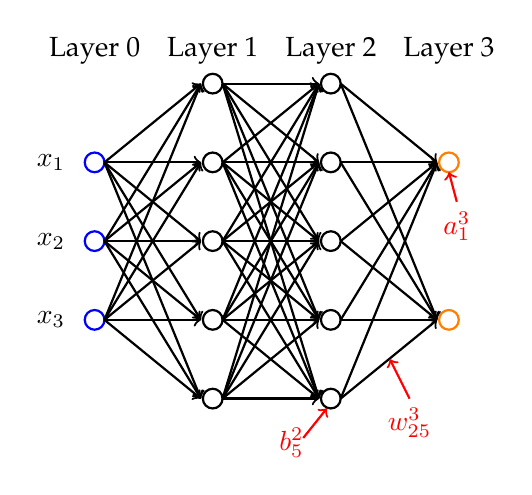
\begin{tikzpicture}[scale=0.5]
		\draw[thick,blue] (0,0) circle [radius=0.25];
		\draw[thick,blue] (0,2) circle [radius=0.25];
		\draw[thick,blue] (0,4) circle [radius=0.25];
		\node[left] at (-0.5,4) {$x_1$};
		\node[left] at (-0.5,2) {$x_2$};
		\node[left] at (-0.5,0) {$x_3$};
		\draw[thick] (3,6) circle [radius=0.25];
		\draw[thick] (3,4) circle [radius=0.25];
		\draw[thick] (3,2) circle [radius=0.25];
		\draw[thick] (3,0) circle [radius=0.25];
		\draw[thick] (3,-2) circle [radius=0.25];
		\draw[thick] (6,6) circle [radius=0.25];
		\draw[thick] (6,4) circle [radius=0.25];
		\draw[thick] (6,2) circle [radius=0.25];
		\draw[thick] (6,0) circle [radius=0.25];
		\draw[thick] (6,-2) circle [radius=0.25];
		\draw[thick,orange] (9,4) circle [radius=0.25];
		\draw[thick,orange] (9,0) circle [radius=0.25];
		\draw[thick,->] (0.25,4) -- (2.7,6);
		\draw[thick,->] (0.25,4) -- (2.7,4);
		\draw[thick,->] (0.25,4) -- (2.7,2);
		\draw[thick,->] (0.25,4) -- (2.7,0);
		\draw[thick,->] (0.25,4) -- (2.7,-2);
		\draw[thick,->] (0.25,2) --(2.7,6);
		\draw[thick,->] (0.25,2) --(2.7,4);
		\draw[thick,->] (0.25,2) --(2.7,2);
		\draw[thick,->] (0.25,2) --(2.7,0);
		\draw[thick,->] (0.25,2) --(2.7,-2);
		\draw[thick,->] (0.25,0) -- (2.7,6);
		\draw[thick,->] (0.25,0) -- (2.7,4);
		\draw[thick,->] (0.25,0) -- (2.7,2);
		\draw[thick,->] (0.25,0) -- (2.7,0);
		\draw[thick,->] (0.25,0) -- (2.7,-2);
		\draw[thick,->] (3.25,-2) -- (5.7,6);
		\draw[thick,->] (3.25,-2) -- (5.7,4);
		\draw[thick,->] (3.25,-2) -- (5.7,2);
		\draw[thick,->] (3.25,-2) -- (5.7,0);
		\draw[thick,->] (3.25,-2) -- (5.7,-2);
		\draw[thick,->] (3.25,0) -- (5.7,6);
		\draw[thick,->] (3.25,0) -- (5.7,4);
		\draw[thick,->] (3.25,0) -- (5.7,2);
		\draw[thick,->] (3.25,0) -- (5.7,0);
		\draw[thick,->] (3.25,0) -- (5.7,-2);
		\draw[thick,->] (3.25,2) -- (5.7,6);
		\draw[thick,->] (3.25,2) -- (5.7,4);
		\draw[thick,->] (3.25,2) -- (5.7,2);
		\draw[thick,->] (3.25,2) -- (5.7,0);
		\draw[thick,->] (3.25,2) -- (5.7,-2);
		\draw[thick,->] (3.25,4) -- (5.7,6);
		\draw[thick,->] (3.25,4) -- (5.7,4);
		\draw[thick,->] (3.25,4) -- (5.7,2);
		\draw[thick,->] (3.25,4) -- (5.7,0);
		\draw[thick,->] (3.25,4) -- (5.7,-2);
		\draw[thick,->] (3.25,6) -- (5.7,6);
		\draw[thick,->] (3.25,6) -- (5.7,4);
		\draw[thick,->] (3.25,6) -- (5.7,2);
		\draw[thick,->] (3.25,6) -- (5.7,0);
		\draw[thick,->] (3.25,6) -- (5.7,-2);
		\draw[thick,->] (6.25,6) -- (8.7,4);
		\draw[thick,->] (6.25,4) -- (8.7,4);
		\draw[thick,->] (6.25,2) -- (8.7,4);
		\draw[thick,->] (6.25,0) -- (8.7,4);
		\draw[thick,->] (6.25,-2) -- (8.7,4);
		\draw[thick,->] (6.25,6) -- (8.7,0);
		\draw[thick,->] (6.25,4) -- (8.7,0);
		\draw[thick,->] (6.25,2) -- (8.7,0);
		\draw[thick,->] (6.25,0) -- (8.7,0);
		\draw[thick,->] (6.25,-2) -- (8.7,0);
		\node[above] at (0,6.25) {Layer 0};
		\node[above] at (3,6.25) {Layer 1};
		\node[above] at (6,6.25) {Layer 2};
		\node[above] at (9,6.25) {Layer 3};
		\node[below,red] at (8,-2) {$w_{25}^3$};
		\draw[thick,red,->] (8,-2) -- (7.5,-1);
		\node[below,red] at (5,-2.5) {$b_{5}^2$};
		\draw[thick,red,->] (5.3,-3) -- (5.9,-2.25);
		\node[below,red] at (9.2,3) {$a_{1}^3$};
		\draw[thick,red,->] (9.2,3) -- (9,3.75);
		\end{tikzpicture}
	\end{center}
	We have the following notations:
	\begin{itemize}
		\item $b_j^{\ell}$ is the bias of the $j$\textsuperscript{th} neuron in the $\ell$\textsuperscript{th} layer.
		\item $a_j^{\ell}$ is the activation of the $j$\textsuperscript{th} neuron in the $\ell$\textsuperscript{th} layer.
		\item $w_{jk}^\ell$ is the weight for the connection from the $k$\textsuperscript{th} neuron in the $(\ell-1)$\textsuperscript{th} layer to the $j$\textsuperscript{th} neuron in the $\ell$\textsuperscript{th} layer.
	\end{itemize}
	If the activation function is $f$ and the loss function we are minimizing is $C$, then the equations describing the network are:
	\begin{align*}
		a_j^\ell&=f\left(\sum_{k}w_{jk}^\ell a_k^{\ell-1}+b_j^\ell\right)\\
		\text{Loss}&=C\left(a^L\right)
	\end{align*}
	Let the weighted inputs to the $d$ neurons in layer $\ell$ be defined as
	$$z^\ell\equiv w^\ell a^{\ell-1}+b^\ell,\quad\text{where }z^\ell\in\mathbb{R}^d.$$
	Then, the activation of layer $\ell$ is also written as $a^\ell\equiv f(z^\ell)$. Also, let $\delta_j^\ell\equiv\frac{\partial C}{\partial z_j^\ell}$ denote the {\it error} of neuron $j$ in layer $\ell$. Then, $\delta^\ell\in\mathbb{R}^d$ denotes the full vector of errors associated with layer $\ell$.
	\item[Equations of Backpropagation] ~
	\begin{align*}
		\delta^L&=\grad_a{C}\odot f'\left(z^L\right)\\
		\delta^\ell&=\left[\left(w^{\ell+1}\right)^\intercal\delta^{\ell+1}\right]\odot f'\left(z^\ell\right)\\
		\dfrac{\partial C}{\partial b_j^\ell}&=\delta_j^\ell\\
		\dfrac{\partial C}{\partial w_{jk}^\ell}&=a_k^{\ell-1}\delta_j^\ell
	\end{align*}
	The symbol $\odot$ represents the Hadamard product.
	\begin{equation*}
		\begin{pmatrix}
			a & b\\
			c & d
		\end{pmatrix} \odot
		\begin{pmatrix}
			e & f\\
			g & h
		\end{pmatrix}=
		\begin{pmatrix}
			ae & bf \\
			cg & dh
		\end{pmatrix}.
	\end{equation*}
\end{description}
\subsection{Recurrent Neural Networks}

\begin{description}
	\item[Temporal/Sequence Problems] ~
	\begin{itemize}
		\item Sequence prediction problems can be recast in a form amenable to feedforward neural networks.
		\item We have to engineer how {\it history} is mapped to a vector (representation). This vector is then fed into, e.g., a neural network.
		\item We would like to learn how to encode the {\it history} into a vector.
	\end{itemize}
	\item[Key Concepts] ~
	\begin{itemize}
		\item {\bf Encoding} -- e.g., mapping a sequence to a vector
		\item {\bf Decoding} -- e.g., mapping a vector to, e.g., a sequence
	\end{itemize}
	\item[Example: Encoding Sentences] ~
	\begin{itemize}[topsep=0pt]
		\item Introduce adjustable {\it lego pieces} and optimize them for end-to-end performance.	
	\begin{center}
		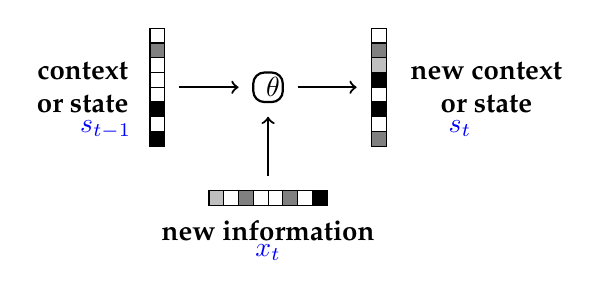
\begin{tikzpicture}[scale=0.75]
		\draw[fill=black] (0,0) rectangle (0.25,0.25);
		\draw[] (0,0.25) rectangle (0.25,0.5);
		\draw[fill=black] (0,0.5) rectangle (0.25,0.75);
		\draw[] (0,0.75) rectangle (0.25,1);
		\draw[] (0,1) rectangle (0.25,1.25);
		\draw[] (0,1.25) rectangle (0.25,1.5);
		\draw[fill=gray] (0,1.5) rectangle (0.25,1.75);
		\draw[] (0,1.75) rectangle (0.25,2);
		\draw[thick,->] (0.5,1) -- (1.5,1);
		\draw[rounded corners, thick] (1.75,0.75) rectangle (2.25,1.25);
		\node[right] at (1.8,1) {$\theta$};
		\node[left, align=center] at (-0.2,1) {\textbf{context} \\ \textbf{or state}};
		\draw[thick,->] (2.5,1) -- (3.5,1);
		\draw[fill=gray] (3.75,0) rectangle (4,0.25);
		\draw[] (3.75,0.25) rectangle (4,0.5);
		\draw[fill=black] (3.75,0.5) rectangle (4,0.75);
		\draw[] (3.75,0.75) rectangle (4,1);
		\draw[fill=black] (3.75,1) rectangle (4,1.25);
		\draw[fill=lightgray] (3.75,1.25) rectangle (4,1.5);
		\draw[fill=gray] (3.75,1.5) rectangle (4,1.75);
		\draw[] (3.75,1.75) rectangle (4,2);
		\draw[thick,->] (2,-0.5) -- (2,0.5);
		\draw[fill=lightgray] (1,-1) rectangle (1.25,-0.75);
		\draw[] (1.25,-1) rectangle (1.5,-0.75);
		\draw[fill=gray] (1.5,-1) rectangle (1.75,-0.75);
		\draw[] (1.75,-1) rectangle (2,-0.75);
		\node[below] at (2,-1.1) {\textbf{new information}};
		\node[below,blue] at (2,-1.5) {$x_t$};
		\draw[] (2,-1) rectangle (2.25,-0.75);
		\draw[fill=gray] (2.25,-1) rectangle (2.5,-0.75);
		\draw[] (2.5,-1) rectangle (2.75,-0.75);
		\draw[fill=black] (2.75,-1) rectangle (3,-0.75);
		\node[right, align=center] at (4.25,1) {\textbf{new context} \\ \textbf{or state}};
		\node[below,blue] at (5.25,0.6) {$s_t$};
		\node[below,blue] at (-0.75,0.6) {$s_{t-1}$};
		\end{tikzpicture}
		$$s_t=\tanh(W^{s,s}s_{t-1} + W^{s,x}x_t)$$
	\end{center}
	\item Let's say we want to encode the incomplete sentence {\bf Efforts and courage are not}. First, we have to represent the first word as a vector (say, a one-hot vector). This will be $x_1$. Then,
	$$s_1=\tanh\left(W^{s,x}x_1\right).$$
	The second word will be $x_2$, and we compute for $s_2$.
	$$s_2=\tanh(W^{s,s}s_1+W^{s,x}x_t).$$
	We continue this process until we've encoded all the words in the sentence. We can visualize this as follows:
	\begin{center}
		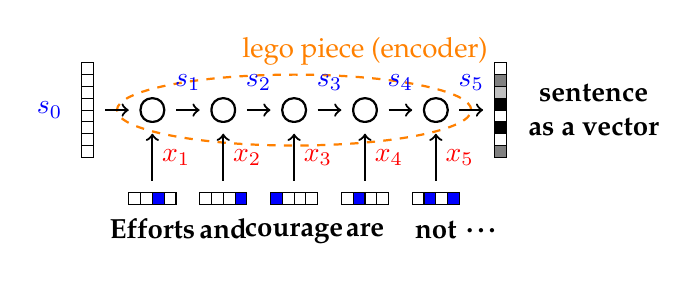
\begin{tikzpicture}[scale=0.6]
		\draw[orange, thick, dashed] (4.5,1) ellipse (3.75 and 0.75);
		\node[above, orange] at (6,1.75) {lego piece (encoder)};
		\draw[] (0,0) rectangle (0.25,0.25);
		\draw[] (0,0.25) rectangle (0.25,0.5);
		\draw[] (0,0.5) rectangle (0.25,0.75);
		\draw[] (0,0.75) rectangle (0.25,1);
		\draw[] (0,1) rectangle (0.25,1.25);
		\draw[] (0,1.25) rectangle (0.25,1.5);
		\draw[] (0,1.5) rectangle (0.25,1.75);
		\draw[] (0,1.75) rectangle (0.25,2);
		\draw[thick,->] (0.5,1) -- (1,1);
		\draw[thick,->] (2,1) -- (2.5,1);
		\draw[thick,->] (3.5,1) -- (4,1);
		\draw[thick,->] (5,1) -- (5.5,1);
		\draw[thick,->] (6.5,1) -- (7,1);
		\draw[thick,->] (8,1) -- (8.5,1);
		\draw[rounded corners, thick] (1.25,0.75) rectangle (1.75,1.25);
		\draw[rounded corners, thick] (2.75,0.75) rectangle (3.25,1.25);
		\draw[rounded corners, thick] (4.25,0.75) rectangle (4.75,1.25);
		\draw[rounded corners, thick] (5.75,0.75) rectangle (6.25,1.25);
		\draw[rounded corners, thick] (7.25,0.75) rectangle (7.75,1.25);
		\node[left, align=center,blue] at (-0.2,1) {$s_0$};
		\node[above, blue] at (2.25,1.2) {$s_1$};
		\node[above, blue] at (3.75,1.2) {$s_2$};
		\node[above, blue] at (5.25,1.2) {$s_3$};
		\node[above, blue] at (6.75,1.2) {$s_4$};
		\node[above, blue] at (8.25,1.2) {$s_5$};
		\node[right, red] at (1.5,0) {$x_1$};
		\node[right, red] at (3,0) {$x_2$};
		\node[right, red] at (4.5,0) {$x_3$};
		\node[right, red] at (6,0) {$x_4$};
		\node[right, red] at (7.5,0) {$x_5$};
		\draw[fill=gray] (8.75,0) rectangle (9,0.25);
		\draw[] (8.75,0.25) rectangle (9,0.5);
		\draw[fill=black] (8.75,0.5) rectangle (9,0.75);
		\draw[] (8.75,0.75) rectangle (9,1);
		\draw[fill=black] (8.75,1) rectangle (9,1.25);
		\draw[fill=lightgray] (8.75,1.25) rectangle (9,1.5);
		\draw[fill=gray] (8.75,1.5) rectangle (9,1.75);
		\draw[] (8.75,1.75) rectangle (9,2);
		\draw[thick,->] (1.5,-0.5) -- (1.5,0.5);
		\draw[thick,->] (3,-0.5) -- (3,0.5);
		\draw[thick,->] (4.5,-0.5) -- (4.5,0.5);
		\draw[thick,->] (6,-0.5) -- (6,0.5);
		\draw[thick,->] (7.5,-0.5) -- (7.5,0.5);
		\draw[] (1,-1) rectangle (1.25,-0.75);
		\draw[] (1.25,-1) rectangle (1.5,-0.75);
		\draw[fill=blue] (1.5,-1) rectangle (1.75,-0.75);
		\draw[] (1.75,-1) rectangle (2,-0.75);
		\node[below] at (1.5,-1.1) {\textbf{Efforts}};
		\node[below] at (3,-1.1) {\textbf{and}};
		\node[below] at (4.5,-1.2) {\textbf{courage}};
		\node[below] at (6,-1.2) {\textbf{are}};
		\node[below] at (7.5,-1.15) {\textbf{not}};
		\node[below] at (8.5,-1.3) {\textbf{\dots}};
		\draw[] (2.5,-1) rectangle (2.75,-0.75);
		\draw[] (2.75,-1) rectangle (3,-0.75);
		\draw[] (3,-1) rectangle (3.25,-0.75);
		\draw[fill=blue] (3.25,-1) rectangle (3.5,-0.75);
		\draw[fill=blue] (4,-1) rectangle (4.25,-0.75);
		\draw[] (4.25,-1) rectangle (4.5,-0.75);
		\draw[] (4.75,-1) rectangle (5,-0.75);
		\draw[] (4.5,-1) rectangle (4.75,-0.75);
		\draw[] (5.5,-1) rectangle (5.75,-0.75);
		\draw[fill=blue] (5.75,-1) rectangle (6,-0.75);
		\draw[] (6,-1) rectangle (6.25,-0.75);
		\draw[] (6.25,-1) rectangle (6.5,-0.75);
		\draw[] (7,-1) rectangle (7.25,-0.75);
		\draw[fill=blue] (7.25,-1) rectangle (7.5,-0.75);
		\draw[] (7.5,-1) rectangle (7.75,-0.75);
		\draw[fill=blue] (7.75,-1) rectangle (8,-0.75);
		\node[right, align=center] at (9.25,1) {\textbf{sentence} \\ \textbf{as a vector}};
		\end{tikzpicture}
	\end{center}
	\end{itemize}
	\item[Differences from standard feedforward architecture] ~
	\begin{itemize}
		\item Input is received at each layer (per word), not just at the beginning as in a typical feedforward network.
		\item The number of layers varies and depends on the length of the sentence.
		\item Parameters of each layer (representing an application of an RNN) are shared (same RNN at each step).
	\end{itemize}
	\item[Basic RNN] ~
	$$s_t=\tanh(W^{s,s}s_{t-1} + W^{s,x}x_t)$$
	\item[Simple Gated RNN] ~
	\begin{align*}
		g_t&=\text{sigmoid}\left(W^{g,s}s_{t-1}+W^{g,x}x_t\right)\\
		s_t&=\left(1-g_t\right)\odot s_{t-1}+g_t\odot\tanh(W^{s,s}s_{t-1}+W^{s,x}x_t)
	\end{align*}
	\item[Long Short-Term Memory (LSTM)] ~
	\begin{alignat*}{2}
		f_t&=\text{sigmoid}\left(W^{f,h}h_{t-1}+W^{f,x}x_t\right)\quad&&\textcolor{red}{\text{forget gate}}\\
		i_t&=\text{sigmoid}\left(W^{i,h}h_{t-1}+W^{i,x}x_t\right) &&\textcolor{red}{\text{input gate}}\\
		o_t&=\text{sigmoid}\left(W^{o,h}h_{t-1}+W^{o,x}x_t\right) &&\textcolor{red}{\text{output gate}}\\
		c_t&=f_t\odot c_{t-1}+i_t\odot\tanh(W^{c,h}h_{t-1}+W^{c,x}x_t) \quad&&\textcolor{red}{\text{memory cell}}\\
		h_t&=o_t\odot\tanh(c_t)&&\textcolor{red}{\text{visible state}}
	\end{alignat*}	
	\item[Markov Language Models] Let $w\in V$ denote the set of possible words/symbols that includes
	\begin{itemize}
		\item an $\mathbf{UNK}$ symbol for any unknown word (out of vocabulary)
		\item $\mathbf{\langle beg\rangle}$ symbol for specifying the start of a sentence
		\item $\mathbf{\langle end\rangle}$ symbol for specifying the end of the sentence
	\end{itemize}
	\item[First-order Markov Model] In a first-order Markov model ({\bf bigram model}), the next symbol only depends on the previous one. Each symbol (except $\langle$beg$\rangle$) in the sequence is predicted using the same condition probability table until an $\langle$end$\rangle$ symbol is seen. The probability associated to the sentence is
	$$\prod_{i=1}\mathbb{P}\left(w_i|w_{i-1}\right).$$
	\item[Maximum Likelihood Estimation] The goal is to maximize the probability that the model can generate all the observed sentences (corpus $S$) $$s\in S, s=\left\{w_1^s,w_2^s,\dots,w_{|s|}^s\right\}$$
	$$\ell=\log\left\{\prod_{s\in S}\left[\prod_{i=1}^{|s|}\mathbb{P}\left(w_i^s|w_{i-1}^s\right)\right]\right\}$$
	The maximum likelihood estimate is obtained as normalized counts of successive word occurrences (matching statistics)
	$$\widehat{\mathbb{P}}\left(w'|w\right)=\dfrac{\text{count}\left(w',w\right)}{\sum\limits_{\widetilde{w}}\text{count}\left(w,\widetilde{w}\right)}$$
	\item[Feature-based Markov Model] We can also represent the Markov model as a feedforward neural network (very extendable). We define a one-hot vector, $\phi\left(w_{i-1}\right)$, corresponding to the previous word. This will be an input to the feedforward neural network.
	\begin{center}
		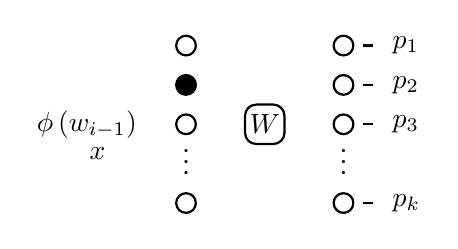
\begin{tikzpicture}[scale=0.5]
		\draw[thick] (0,4) circle [radius=0.25];
		\draw[thick,fill=black] (0,3) circle [radius=0.25];
		\draw[thick] (0,2) circle [radius=0.25];		
		\draw[thick] (0,0) circle [radius=0.25];		
		\node[left] at (-1,2) {$\phi\left(w_{i-1}\right)$};
		\node[left] at (-1.8,1.25) {$x$};
		\node[] at (0,1.25) {$\vdots$};
		\node[] at (4,1.25) {$\vdots$};
		\node[] at (2,2) {$W$};
		\draw[rounded corners, thick] (1.5,1.5) rectangle (2.5,2.5);
		\draw[thick] (4,4) circle [radius=0.25];
		\draw[thick] (4,3) circle [radius=0.25];
		\draw[thick] (4,2) circle [radius=0.25];
		\draw[thick] (4,0) circle [radius=0.25];
		\draw[thick] (4.5,0) -- (4.75,0);
		\draw[thick] (4.5,2) -- (4.75,2);
		\draw[thick] (4.5,3) -- (4.75,3);
		\draw[thick] (4.5,4) -- (4.75,4);
		\node[right] at (5,4) {$p_1$};
		\node[right] at (5,3) {$p_2$};
		\node[right] at (5,2) {$p_3$};
		\node[right] at (5,0) {$p_k$};
		\end{tikzpicture}
	\end{center}
	In the figure, 
	$$p_k=\mathbb{P}\left(w_i=k|w_{i-1}\right)$$
	is the probability of the next word, given the previous word. The aggregate input to the $k$\textsuperscript{th} output unit is
	$$z_k=\sum_{k}x_jW_{jk}+W_{0k}.$$
	These input values are not probabilities. A typical transformation is the {\bf softmax transformation}:
	$$p_k=\dfrac{e^{z_k}}{\sum\limits_{j}e^{z_j}}.$$
	\item[RNNs for Sequences] Our RNN now also produces an output (e.g., a word) as well as update its state
	\begin{center}
		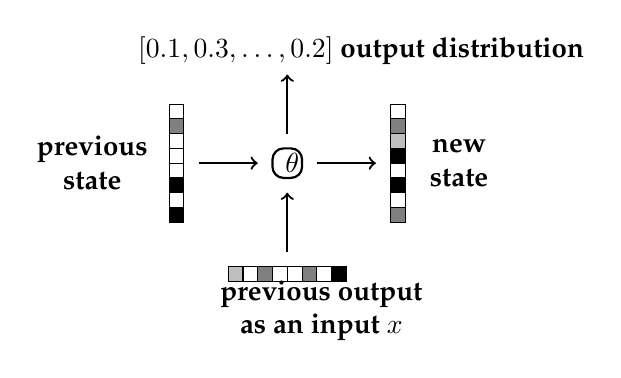
\begin{tikzpicture}[scale=0.75]
		\draw[fill=black] (0,0) rectangle (0.25,0.25);
		\draw[] (0,0.25) rectangle (0.25,0.5);
		\draw[fill=black] (0,0.5) rectangle (0.25,0.75);
		\draw[] (0,0.75) rectangle (0.25,1);
		\draw[] (0,1) rectangle (0.25,1.25);
		\draw[] (0,1.25) rectangle (0.25,1.5);
		\draw[fill=gray] (0,1.5) rectangle (0.25,1.75);
		\draw[] (0,1.75) rectangle (0.25,2);
		\draw[thick,->] (0.5,1) -- (1.5,1);
		\draw[rounded corners, thick] (1.75,0.75) rectangle (2.25,1.25);
		\node[right] at (1.8,1) {$\theta$};
		\node[left, align=center] at (-0.2,1) {\textbf{previous} \\ \textbf{state}};
		\draw[thick,->] (2.5,1) -- (3.5,1);
		\draw[fill=gray] (3.75,0) rectangle (4,0.25);
		\draw[] (3.75,0.25) rectangle (4,0.5);
		\draw[fill=black] (3.75,0.5) rectangle (4,0.75);
		\draw[] (3.75,0.75) rectangle (4,1);
		\draw[fill=black] (3.75,1) rectangle (4,1.25);
		\draw[fill=lightgray] (3.75,1.25) rectangle (4,1.5);
		\draw[fill=gray] (3.75,1.5) rectangle (4,1.75);
		\draw[] (3.75,1.75) rectangle (4,2);
		\draw[thick,->] (2,-0.5) -- (2,0.5);
		\draw[fill=lightgray] (1,-1) rectangle (1.25,-0.75);
		\draw[] (1.25,-1) rectangle (1.5,-0.75);
		\draw[fill=gray] (1.5,-1) rectangle (1.75,-0.75);
		\draw[] (1.75,-1) rectangle (2,-0.75);
		\node[right, align=center] at (0.7,-1.5) {\textbf{previous output} \\ \textbf{as an input} $x$};
		\draw[] (2,-1) rectangle (2.25,-0.75);
		\draw[fill=gray] (2.25,-1) rectangle (2.5,-0.75);
		\draw[] (2.5,-1) rectangle (2.75,-0.75);
		\draw[fill=black] (2.75,-1) rectangle (3,-0.75);
		\node[right, align=center] at (4.25,1) {\textbf{new} \\ \textbf{state}};
		\draw[thick,->] (2,1.5) -- (2,2.5);
		\node[above] at (3.25,2.5) {$[0.1,0.3,\dots,0.2]$ \textbf{output distribution}};
		\end{tikzpicture}
	\end{center}
	\begin{alignat*}{2}
		s_t&=\tanh(W^{s,s}s_{t-1}+W^{s,x}x_t)\quad&&\textcolor{red}{\text{state}}\\
		p_t&=\text{softmax}\left(W^os_t\right)&&\textcolor{red}{\text{output distribution}}
	\end{alignat*}
	\item[Decoding] ~
	\begin{center}
		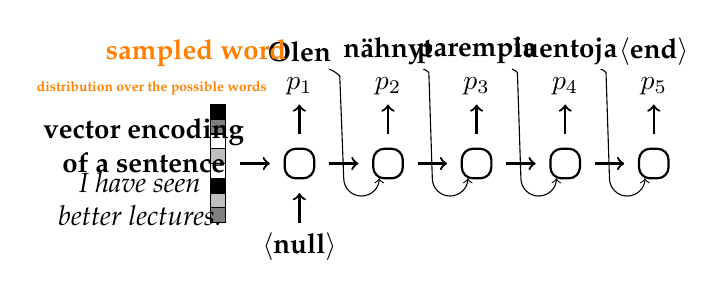
\begin{tikzpicture}[scale=0.75]
		\draw[fill=gray] (0,0) rectangle (0.25,0.25);
		\draw[fill=lightgray] (0,0.25) rectangle (0.25,0.5);
		\draw[fill=black] (0,0.5) rectangle (0.25,0.75);
		\draw[] (0,0.75) rectangle (0.25,1);
		\draw[fill=lightgray] (0,1) rectangle (0.25,1.25);
		\draw[] (0,1.25) rectangle (0.25,1.5);
		\draw[fill=gray] (0,1.5) rectangle (0.25,1.75);
		\draw[fill=black] (0,1.75) rectangle (0.25,2);
		\draw[thick,->] (0.5,1) -- (1,1);
		\draw[thick,->] (2,1) -- (2.5,1);
		\draw[thick,->] (3.5,1) -- (4,1);
		\draw[thick,->] (5,1) -- (5.5,1);
		\draw[thick,->] (6.5,1) -- (7,1);
		\draw[rounded corners, thick] (1.25,0.75) rectangle (1.75,1.25);
		\draw[rounded corners, thick] (2.75,0.75) rectangle (3.25,1.25);
		\draw[rounded corners, thick] (4.25,0.75) rectangle (4.75,1.25);
		\draw[rounded corners, thick] (5.75,0.75) rectangle (6.25,1.25);
		\draw[rounded corners, thick] (7.25,0.75) rectangle (7.75,1.25);
		\node[below] at (1.5,0) {\textbf{$\langle$null$\rangle$}};
		\node[above] at (1.5,2.55) {\textbf{Olen}};
		\node[above] at (3,2.5) {\textbf{n\"ahnyt}};
		\node[above] at (4.5,2.53) {\textbf{parempia}};
		\node[above] at (6,2.5) {\textbf{luentoja}};
		\draw[->] (2,2.6) arc(70:45:0.5) -- (2.25,0.75) arc(180:360:0.3);
		\draw[->] (3.6,2.6) arc(70:45:0.25) -- (3.75,0.75) arc(180:360:0.3);
		\draw[->] (5.1,2.6) arc(70:45:0.25) -- (5.25,0.75) arc(180:360:0.3);
		\draw[->] (6.6,2.6) arc(70:45:0.25) -- (6.75,0.75) arc(180:360:0.3);
		\node[above, orange] at (-0.25,2.48) {\textbf{sampled word}};
		\node[above, orange] at (-1,2) {\textbf{\tiny distribution over the possible words}};
		\node[above] at (7.5,2.5) {$\langle$\textbf{end}$\rangle$};
		\node[above] at (1.5,2) {$p_1$};
		\node[above] at (3,2) {$p_2$};
		\node[above] at (4.5,2) {$p_3$};
		\node[above] at (6,2) {$p_4$};
		\node[above] at (7.5,2) {$p_5$};
		\draw[thick,->] (1.5,0) -- (1.5,0.5);
		\draw[thick,->] (1.5,1.5) -- (1.5,2);
		\draw[thick,->] (3,1.5) -- (3,2);
		\draw[thick,->] (4.5,1.5) -- (4.5,2);
		\draw[thick,->] (6,1.5) -- (6,2);
		\draw[thick,->] (7.5,1.5) -- (7.5,2);
		\node[right, align=center] at (-3,1.3) {\textbf{vector encoding} \\ \textbf{of a sentence}};
		\node[right, align=center] at (-2.75,0.4) {\textit{I have seen} \\ \textit{better lectures.}};
		\end{tikzpicture}
	\end{center}
\end{description}

\subsection{Convolutional Neural Networks}

\begin{description}
	\item[Problem] Image classification
	\begin{itemize}
		\item The presence of objects may vary in location across different images.
	\end{itemize}
	\item[Patch classifier/filter] ~
	\begin{center}
		\begin{tikzpicture}
		\node[inner sep=0pt]  at (0,1)
		{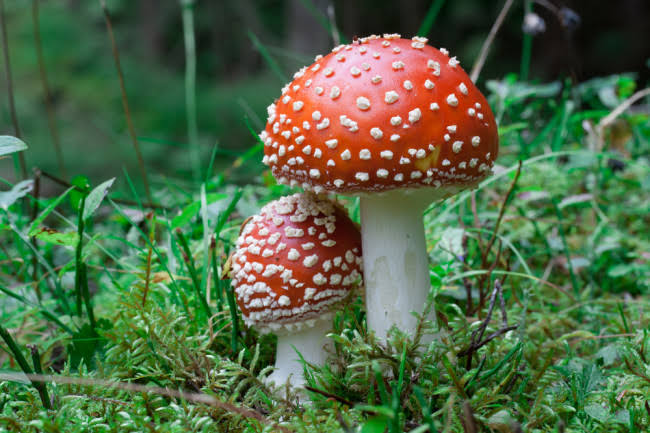
\includegraphics[width=0.25\columnwidth]{mushroom.jpeg}};
		\node[inner sep=0pt]  at (4,1)
		{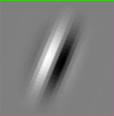
\includegraphics[width=0.35in]{filter.png}};
		\draw[red] (-0.1,1.3) -- (2.97,1.47);
		\draw[red] (-0.1,1.1) -- (2.97,0.53);
		\node[inner sep=0pt]  at (2.5,1) {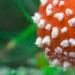
\includegraphics[width=0.1\columnwidth]{mushroom2.jpeg}};
		\draw[red] (-0.3,1.1) rectangle (-0.1,1.3);
		\draw[red] (2.03,0.53) rectangle (2.97,1.47);
		\draw[red] (-0.3,1.1) -- (2.03,0.53);
		\draw[red] (-0.3,1.3) -- (2.03,1.47);
		\node[] at (2.5,0.25) {input};
		\node[] at (4,0.25) {weights};
		\draw[step=0.094,black,thin] (3.54,0.53) grid (4.48,1.47);
		\end{tikzpicture}
	\end{center}
	The patch classifier goes through the entire image. We can think of the weights as the image that the unit prefers to see.
	\item[Convolution] The convolution is an operation between two functions $f$ and $g$:
	$$\left(f*g\right)(t)\equiv\int_{-\infty}^{+\infty}f(\tau)g(t-\tau)d\tau.$$
	Intuitively, convolution {\it blends} the two functions $f$ and $g$ by expressing the amount of overlap of one function as it is shifted over another function.
	\item[Discrete Convolution] For discrete functions, we can define the convolution as
	$$\left(f*g\right)[n]\equiv\sum_{m=-\infty}^{m=+\infty}f[m]g[n-m].$$
	\item[Pooling] We wish to know whether a feature was there but not exactly where it was.
	\item[Pooling (Max)] Pooling region and {\it stride} may vary.
	\begin{itemize}
		\item Pooling induces translation invariance at the cost of spatial resolution.
		\item Stride reduces the size of the resulting feature map.
	\end{itemize}
	\begin{center}
		\begin{tikzpicture}
		\node[inner sep=0pt]  at (0,1)
		{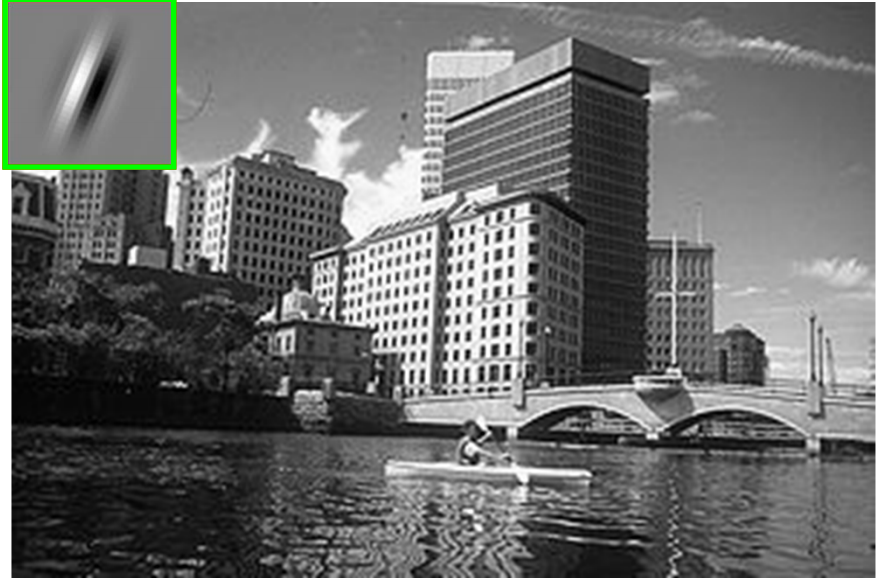
\includegraphics[width=1.25in]{orig.png}};
		\node[inner sep=0pt]  at (3.25,1)
		{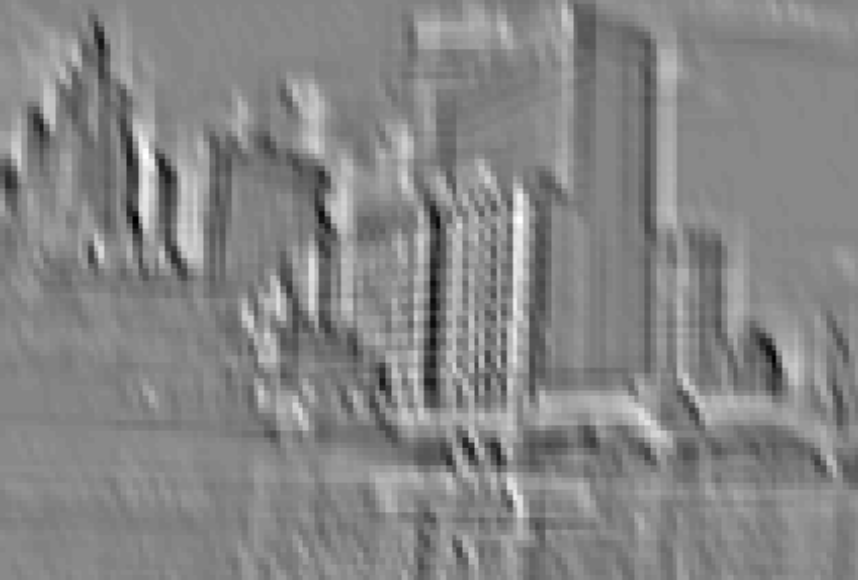
\includegraphics[width=1.22in]{fmap.png}};
		\node[inner sep=0pt]  at (6,1) {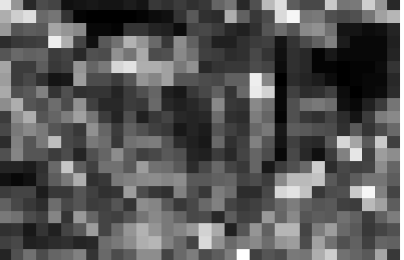
\includegraphics[width=0.75in]{maxpool.png}};
		\node[below] at (0,-0.25) {original};
		\node[below] at (3.25,-0.25) {feature map};
		\node[below, align=center] at (6,0) {feature map \\ after max pooling};
		\end{tikzpicture}
	\end{center}
	\item[Example of CNN] From LeCun (2013)
	\begin{center}
		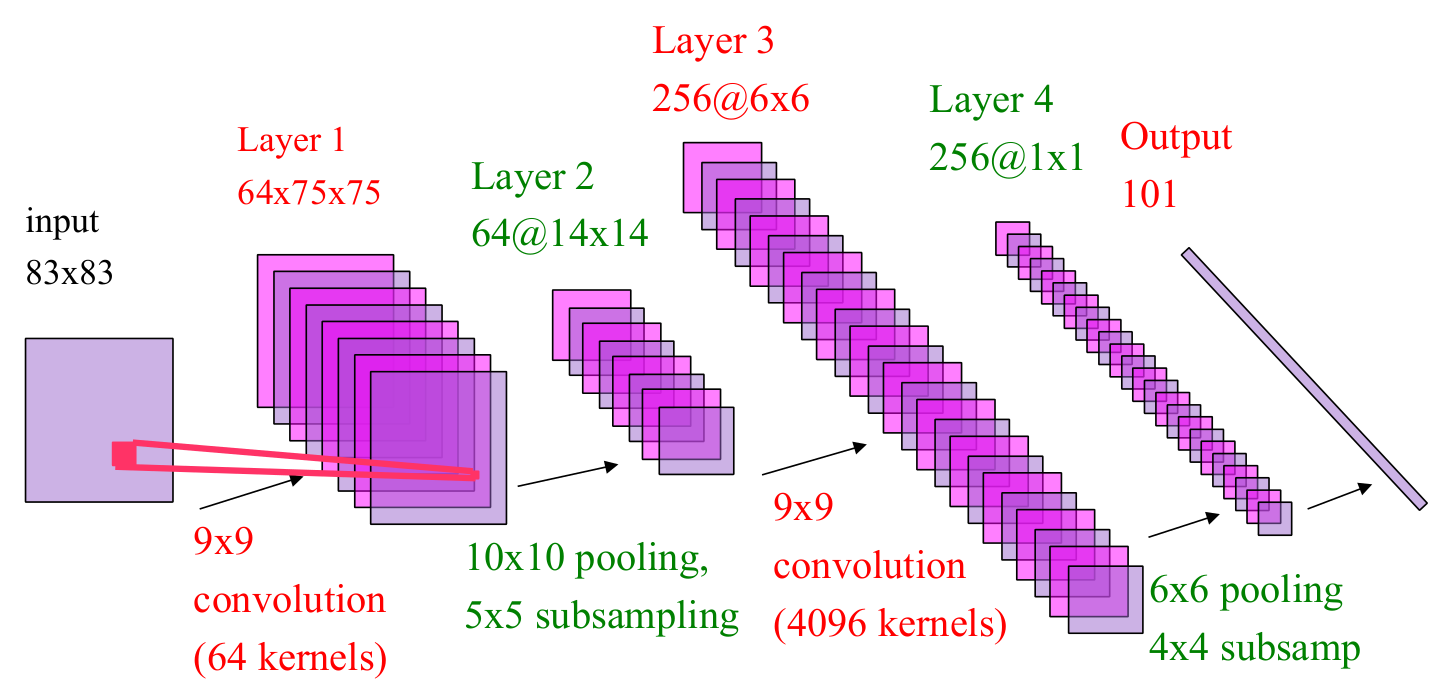
\includegraphics[width=\columnwidth]{cnn.png}
	\end{center}
\end{description}


\section{Unsupervised Learning}\smallskip \hrule height 1pt \smallskip

\subsection{Clustering}

\begin{description}
	\item[Training set] We are provided a training set but with no labels
	$$S_n=\left\{\left.x^{(i)}\right| i=1,\dots,n\right\}$$
	and the goal is to find structure in the data.
	\item[Example: Google News] ~
	\begin{center}
		\includegraphics*[width=0.75\columnwidth]{gnews.png}
	\end{center}
	\item[Example: Image Quantization] ~
	\begin{center}
		\begin{tikzpicture}
		\node[inner sep=0pt]  at (0,1.6)
		{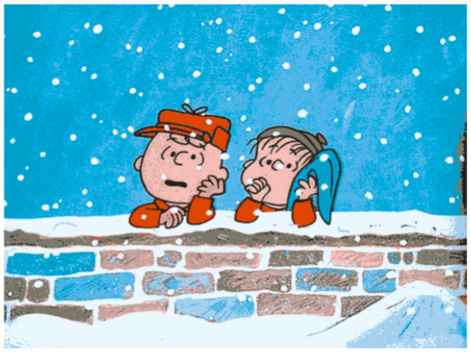
\includegraphics[width=1.5in]{imq1.jpg}};
		\node[inner sep=0pt]  at (4,1.6)
		{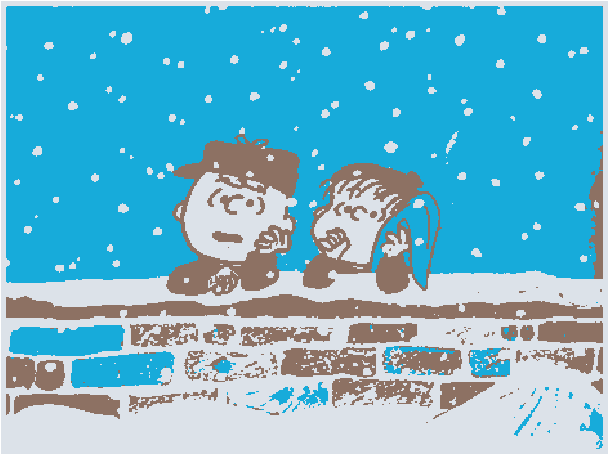
\includegraphics[width=1.5in]{imq2.png}};
		\node[] at (0,0) {original};
		\node[] at (4,0) {compressed};
		\end{tikzpicture}
	\end{center}
	\item[Partition] A partition of a set is a grouping of the set's elements into non-empty subsets, in such a way that {\bf every} element is included in one and only one of the subsets. In other words, $C_1,\dots,C_K$ is a partition of $\{1,\dots,n\}$ if and only if $$C_1\cup\dots\cup C_K=\{1,\dots,n\}\qquad\text{and}$$
	$$C_i\cap C_j=\emptyset\quad\text{for any}\quad i\neq j\quad\text{in}\quad\{1,\dots,K\}.$$
	\item[Clustering: Input] ~
	\begin{itemize}[]
		\item Set of feature vectors $S_n=\left\{\left.x^{(i)}\right|i=1,\dots,n\right\}$
		\item The number of clusters $K$
	\end{itemize}
	\item[Clustering: Output] ~
	\begin{itemize}[]
		\item A partition of indices $\left\{1,\dots,n\right\}$ into $K$ sets, $C_1,\dots,C_K$
		\item {\it Representatives} in each of the $K$ partition sets, given as $z_1,\dots,z_K$
	\end{itemize}
	\item[Cost] We can calculate the total cost by summing the cost of each cluster:
	$$\text{Cost}\left(C_1,\dots,C_K\right)=\sum_{j=1}^{K}\text{Cost}\left(C_j\right)$$
	\item[Similarity Measure] We use the Euclidean distance between the elements of a cluster and its representative to calculate the cost for each cluster. Then, the total cost is
	$$\text{Cost}\left(C_1,\dots,C_K,z_1,\dots,z_K\right)=\sum_{j=1}^{K}\sum_{i\in C_j}\norm{x^{(i)}-z_j}^2.$$
	\item[$K$-Means Algorithm] ~
	\begin{enumerate}
		\item Randomly select $z_1,\dots,z_K$.
		\item Iterate:
		\begin{enumerate}
			\item Given $z_1,\dots,z_K$, assign each data point $x^{(i)}$ to the closest $z_j$ so that
			$$\text{Cost}\left(z_1,\dots,z_K\right)=\sum_{i=1}^{n}\min\limits_{j=1,\dots,K}\norm{x^{(i)}-z_j}^2.$$
			\item Given $C_1,\dots,C_K$, find the best representatives $z_1,\dots,z_K$, i.e., find $z_1,\dots,z_K$ such that
			$$z_j=\argmin\limits_{z}\sum_{i\in C_j}\norm{x^{(i)}-z}^2=\dfrac{1}{\left|C_j\right|}\sum\limits_{i\in C_j}x^{(i)}.$$
		\end{enumerate}
	\end{enumerate}
	\item[$K$-Medoids Algorithm] The $K$-Medoids algorithm is a variation of the $K$-Means algorithm that addresses some of the $K$-Means algorithm's limitations.
	\begin{enumerate}
		\item Randomly select $\left\{z_1,\dots,z_K\right\}\subseteq\left\{x_1,\dots,x_n\right\}$.
		\item Iterate:
		\begin{enumerate}
			\item Given $z_1,\dots,z_K$, assign each $x^{(i)}$ to the closest $z_j$ so that
			$$\text{Cost}\left(z_1,\dots,z_K\right)=\sum_{i=1}^{n}\min\limits_{j=1,\dots,K}\text{dist}\left(x^{(i)},z_j\right)$$
			\item Given $C_j\in\left\{C_1,\dots,C_K\right\}$, find the best representative $z_j\in\left\{x_1,\dots,x_n\right\}$ such that
			$$\sum\limits_{x^{(i)}\in C_j}\text{dist}\left(x^{(i)},z_j\right)$$
			is minimal.
		\end{enumerate}
	\end{enumerate}
\end{description}

\subsection{Generative Models}
\begin{description}
	\item[Generative vs. Discriminative Models] {\it Generative models} work by explicitly modeling the probability distribution of each of the individual classes in the training data. {\it Discriminative models} learn explicit decision boundary between classes.
	\item[Simple Multinomial Generative Model] Consider a multinomial model $M$ to generate text documents. Assume that $M$ has a fixed vocabulary $W$ and we generate a document by sampling one word at a time from this vocabulary. Furthermore, all the words that are generated by $M$ are independent of each other. We denote the probability that $M$ generates certain word $w\in W$ is
	$$\mathbb{P}\left(w|\theta\right)=\theta_w,\quad\theta_w\geq0,\sum_{w\in W}\theta_w=1.$$
	Then, the probability of generating the document $D$ is
	$$\mathbb{P}\left(D|\theta\right)=\prod_{i=1}^{n}\theta_{w_i}=\prod_{w\in W}\theta_w^{\,\text{count}(w)}.$$
	\item[Maximum Likelihood Estimate] The log-likelihood for the model is
	$$\ell=\log\mathbb{P}(D|\theta)=\sum_{w\in W}\text{count}(w)\log\theta_w$$
	and the maximum likelihood estimate is
	$$\widehat{\theta}_w=\dfrac{\text{count}(w)}{\sum\limits_{w'\in W}\text{count}(w')}.$$
	\item[Prediction] Consider using a multinomial generative model $M$ for the task of binary classification consisting of two classes: $+$ (positive class) and $-$ (negative class).
	\begin{itemize}
		\item $\theta^+$: parameter for the positive class
		\item $\theta^-$: parameter for the negative class
	\end{itemize}
	Suppose that we classify a new document $D$ to belong to the positive class if and only if
	$$\log\dfrac{\mathbb{P}(D|\theta^+)}{\mathbb{P}(D|\theta^-)}\geq0.$$
	The generative classifier is equivalent to a linear classifier:
	$$\log\dfrac{\mathbb{P}(D|\theta^+)}{\mathbb{P}(D|\theta^-)}=\sum_{w\in W}\text{count}(w)\log\dfrac{\theta_w^+}{\theta_w^-}=\sum_{w\in W}\text{count}(w)\,\theta'_w.$$
	\item[Prior, Posterior and Likelihood] In the above discussion, there is an assumption that the likelihood of being in one of the classes is the same. However, we may have some prior knowledge and we want to incorporate it into our model. The posterior distribution for the positive class is then
	$$\mathbb{P}\left(y=+|D\right)=\dfrac{\mathbb{P}(D|\theta^+)\,\mathbb{P}(y=+)}{\mathbb{P}(D)}.$$
	The generative classifier becomes
	$$\log\dfrac{\mathbb{P}\left(y=+|D\right)}{\mathbb{P}\left(y=-|D\right)}=\sum_{w\in W}\text{count}(w)\,\theta'_w+\theta'_0$$
	where $\theta'_w=\log\dfrac{\theta^+_w}{\theta^-_w}$ and $\theta'_0=\log\dfrac{\mathbb{P}(y=+)}{\mathbb{P}(y=-)}$.
	\item[Gaussian Generative Models] The likelihood of $\mathbf{x}\in\mathbb{R}^d$ being generated by a Gaussian with mean $\mu$ and standard deviation $\sigma$ is
	$$f_X\left(\mathbf{x}|\mu,\sigma^2\right)=\dfrac{1}{\left(2\pi\sigma^2\right)^{d/2}}\exp(-\dfrac{1}{2\sigma^2}\norm{\mathbf{x}-\mu}^2).$$
	\item[MLE for the Mean] ~
	$$\widehat{\mu}=\frac{1}{n}\sum_{i=1}^{n}\mathbf{x}^{(i)}$$
	\item[MLE for the Variance] ~
	$$\widehat{\sigma}^2=\frac{1}{nd}\sum_{i=1}^{n}\norm{\mathbf{x}^{(i)}-\mu}^2$$
\end{description}

\subsection{Mixture Models; EM Algorithm}
\begin{description}
	\item[Gaussian Mixture Models] Instead of just a single Gaussian, we have a mixture of Gaussian components. Assume that there are $K$ Gaussians with known means and variances. Assume also that the mixture weights $p_1,\dots,p_K$ are known. The likelihood for an observation $\mathbf{x}$ obtained from the model is
	$$p(\mathbf{x}|\theta)=\sum_{j=1}^{K}p_j\mathcal{N}\left(\mathbf{x};\mu^{(j)},\sigma_j^2\mathbf{I}\right).$$
	For the training set
	$$S_n=\left\{\mathbf{x}^{(i)}, i=1,\dots,n\right\},$$
	the likelihood is
	$$\mathbb{P}\left(S_n|\theta\right)=\prod_{i=1}^{n}\sum_{j=1}^{K}p_j\mathcal{N}\left(\mathbf{x}^{(i)};\mu^{(j)},\sigma_j^2\mathbf{I}\right).$$
	\item[Observed Case] Consider the case of hard clustering, i.e., a point either belongs to a cluster or not. Let
	$$\delta(j|i)=
	\begin{cases}
		1,\quad&\mathbf{x}^{(i)}\text{ is assigned to }j\\
		0,&\text{otherwise}.
	\end{cases}$$
	Also, let $\widehat{n}_j=\sum\limits_{i=1}^{n}\delta(j|i)$ denote the number of points belonging to cluster $j$. Maximizing the likelihood gives
	\begin{align*}
		\widehat{p}_j&=\dfrac{\widehat{n}_j}{n}\\
		\widehat{\mu}^{(j)}&=\dfrac{1}{\widehat{n}_j}\sum_{i=1}^{n}\delta(j|i)\,\mathbf{x}^{(i)}\\
		\widehat{\sigma}^2_j&=\dfrac{1}{\widehat{n}_jd}\sum_{i=1}^{n}\delta(j|i)\,\norm{\mathbf{x}^{(i)}-\mu^{(j)}}^2.
	\end{align*}
	\item[The EM Algorithm] Instead of hard clustering, the data can actually be generated from different clusters with different probabilities. We have soft clustering. We can maximize the likelihood through the EM algorithm.
	\begin{enumerate}
		\item[] Randomly initialize $\theta$: $\mu^{(1)},\dots,\mu^{(K)},\sigma^2_1,\dots,\sigma^2_K,p_1,\dots,p_K.$
		\item {\bf E-step:}
		$$p(j|i)=\dfrac{p_j\mathcal{N}\left(\mathbf{x}^{(i)};\mu^{(j)},\sigma^2_j\mathbf{I}\right)}{p\left(\mathbf{x}|\theta\right)}$$
		where $p(\mathbf{x}|\theta)=\sum\limits_{j=1}^{K}p_j\mathcal{N}\left(\mathbf{x}^{(i)};\mu^{(j)},\sigma^2_j\mathbf{I}\right)$
		\item {\bf M-step:}
		\begin{align*}
			\widehat{n}_j&=\sum_{i=1}^{n}p(j|i)\\
			\widehat{p}_j&=\dfrac{\widehat{n}_j}{n}\\
			\widehat{\mu}^{(j)}&=\dfrac{1}{\widehat{n}_j}\sum_{i=1}^{n}p(j|i)\,\mathbf{x}^{(i)}\\
			\widehat{\sigma}^2_j&=\dfrac{1}{\widehat{n}_jd}\sum_{i=1}^{n}p(j|i)\norm{\mathbf{x}^{(i)}-\mu^{(j)}}^2.
		\end{align*}
	\end{enumerate}
\end{description}

\section{Reinforcement Learning}\smallskip \hrule height 1pt \smallskip

\begin{description}
	\item[Objectives of RL] The goal of RL is to learn a good policy with no or limited supervision.
\end{description}

\subsection{Markov Decision Processes}

\begin{description}
	\item[Definition] A {\bf Markov decision process (MDP)} is defined by
	\begin{itemize}
		\item a set of {\bf states} $s\in S$ (may be observed or unobserved);
		\item a set of {\bf actions} $a\in A$;
		\item action-dependent {\bf transition probabilities} $T(s,a,s')=\mathbb{P}(s'|s,a)$ so that, for each state $s$ and action $a$,
		$$\sum_{s'\in S}T(s,a,s')=1$$.
		\item {\bf reward functions} $R(s,a,s')$, representing the reward for starting in state $s$, taking action $a$ and ending up in state $s'$ after one step. (The reward function may also depend only on $s$, or only $s$ and $s$.)
	\end{itemize}
	\item[Property] MDPs satisfy the {\bf Markov property} in that the transition probabilities and rewards depend only on the current state and action, and remain unchanged regardless of the history (i.e., past states and actions) that leads to the current state.
	\item[Utility Function] The main problem for MDPs is to optimize the agent's behavior. We first need to specify the criterion that we are trying to maximize in terms of accumulated rewards. We define a {\bf utility function} and maximize its expectation.
	\begin{itemize}
		\item {\bf Finite horizon based utility:} The utility function is the sum of rewards after acting for a fixed number $n$ of steps. When the rewards depend only on the states, the utility function is
		$$U[s_0,s_1,\dots,s_n]=\sum_{i=0}^{n}R(s_i.)$$
		\item {\bf (Infinite horizon) discounted reward based utility:} In this setting, the reward one step into the future is discounted by a factor $\gamma$, the reward two steps ahead by $\gamma^2$, and so on. The goal is to continue acting (without an end) while maximizing the expected discounted reward. The discounting allows us to focus on near term rewards, and control this focus by changing $\gamma$. If the rewards depend only on the states, the utility function is
		$$U[s_0,s_1,\dots]=\sum_{k=0}^{\infty}\gamma^kR(s_k).$$ 
	\end{itemize}
	\item[Optimal Policy] A {\bf policy} is a function $\pi:S\rightarrow A$ that assigns an action $\pi(s)$ to any state $s$. Given an MDP and a utility function $U[s_0,s_1,\dots,s_n]$, our goal is to find an {\bf optimal policy} function that maximizes the expectation of the utility. We denote the optimal policy by $\pi^*$.
\end{description}

\subsection{Bellman Equations}

\begin{description}
	\item[Value Function] Denote by $Q^*(s,a)$ the expected reward starting at $s$, taking action $a$ and acting optimally. The {\it value function} $V^*(s)$ is the expected reward starting at state $s$ and acting optimally.
	\item[The Bellman Equations] These equations connect the notion of the value of a state and the value of policy.
	\begin{align*}
		V^*(s)&=\max\limits_{a}Q^*(s,a)=Q^*(s,\pi^*(s))\\
		Q^*(s,a)&=\sum_{s'}T(s,a,s')\left[R(s,a,s')+\gamma V^*(s')\right]
	\end{align*}
	We can define the $V^*(s)$ recursively to get
	$$V^*(s)=\max\limits_{a}\left\{\sum_{s'}T(s,a,s')\left[R(s,a,s')+\gamma V^*(s')\right]\right\}$$
\end{description}

\subsection{Value Iteration Algorithm}

\begin{description}
	\item[Definition] {\it Value iteration} is an iterative algorithm that computes the values of states indexed by $k$. Let $V^*_k(s)$ be the expected reward from state $s$ after $k$ steps:
	$$V^*_k(s)\rightarrow V^*(s)\quad\text{as}\quad k\rightarrow\infty.$$
	\begin{enumerate}
		\item Initialization: $V^*_0(s)=0$
		\item Iterate until $V^*_k(s)\simeq V^*_{k+1}(s)\;\forall s$
		$$V^*_{k+1}(s)\leftarrow\max\limits_{a}\left\{\sum_{s'}T(s,a,s')\left[R(s,a,s')+\gamma V^*_k(s')\right]\right\}$$
		\item Compute $Q^*(s,a)$ and $\pi^*(s,a)=\argmax\limits_{a}Q^*(s,a)$.
	\end{enumerate}
	\item[Convergence] This algorithm will converge as long as $\gamma<1$.
\end{description}

\subsection{Q-Value Iteration}
\begin{description}
	\item[Definition] We can directly operate at the level of Q-values. Q-value iteration is a reformulation of value iteration algorithm.
	\item[Update Rule] ~
	$$Q^*_{k+1}(s,a)\leftarrow\sum_{s'}T(s,a,s')\left[R(s,a,s')+\gamma\max\limits_{a'}Q^*_k(s',a')\right]$$
\end{description}

\subsection{Reinforcement Learning}
\begin{description}
	\item[MDP vs. RL] In MDPs, we are given 4 quantities $\langle S,A,T,R\rangle$. In reinforcement learning, we are given only the states and actions $\langle S,A\rangle$. In the real world, transitions and rewards might not be directly available and they need to be estimated.
	\item[Estimation] Consider a random variable $X$. The goal is to estimate
	$$\mathbb{E}\left[f(X)\right]=\sum_{x}p(x)f(x).$$
	We have access to $K$ samples: $x_i$, $i=1,\dots,K$.
	\item[Model-based Learning] ~
	\begin{align*}
		\widehat{p}(x_i)&=\frac{1}{K}\,\text{count}(x_i)\\
		\mathbb{E}\left[f(X)\right]&\approx\sum_{i=1}^{K}\widehat{p}(x_i)f(x_i)
	\end{align*}
	\item[Model-free Learning] ~
	$$\mathbb{E}\left[f(X)\right]\approx\frac{1}{K}\sum_{i=1}^{K}f(x_i)$$
	\item[Q-Value Iteration for RL] ~
	\begin{enumerate}
		\item Initialization: $Q(s,a)=0\;\forall s,a$
		\item Iterate until convergence:
		\begin{enumerate}
			\item Collect sample: $s,a,s',R(s,a,s')$
			\item Update:
			\begin{align*}
				Q_{i+1}(s,a)&\leftarrow\,\alpha\left[R(s,a,s')+\gamma\max\limits_{a'}Q_i(s',a')\right]+(1-\alpha)\,Q_i(s,a)\\
				&=Q_i(s,a)+\alpha\left[R(s,a,s')+\gamma\max\limits_{a'}Q_i(s',a')-Q_i(s,a)\right]
			\end{align*}
		\end{enumerate}
	\end{enumerate}
	
\end{description}



\section{Recommended Resources} \smallskip \hrule height 1pt \smallskip

\bigskip

\begin{itemize}
\item Introduction to Machine Learning with Python (M\"uller and Guido)
\item Machine Learning with Python -- From Linear Models to Deep Learning [Lecture Slides] (\url{http://www.edx.org})
\item LaTeX File (\texttt{\href{https://github.com/mynameisjanus/686xMachineLearning}{github.com/mynameisjanus/686xMachineLearning}})
\end{itemize}

\begin{center}\emph{Please share this cheatsheet with friends!}\end{center}

\end{multicols*}



\end{document}
